\documentclass[10pt]{report}

% ---------- Package Setup ----------
\usepackage[utf8]{inputenc}
\usepackage{amsmath, amssymb}
\usepackage{graphicx}
\usepackage{cite}
\usepackage{hyperref}
\usepackage{geometry}
\usepackage{titlesec}
\usepackage{caption}
\usepackage{subcaption}
\usepackage{tocloft}
\usepackage{xcolor}
\usepackage{booktabs}
\usepackage{algorithm}
\usepackage{algpseudocode}
\usepackage{setspace}
\usepackage{soul}


\newcommand{\rs}[1]{\noindent{\color{red}\textbf{RS:} #1}}
% \newcommand{\hl}[1]{\noindent{\color{blue}\textbf{HL:} #1}}
\newcommand{\rev}[1]{\textcolor{red}{#1}}
\newcommand{\mm}[1]{\noindent{\color{cyan}\textbf{MM:} #1}}

\setstretch{1.5}


\hypersetup{
    colorlinks=true,
    linkcolor=black,
    citecolor=black,
    urlcolor=black
}


% ---------- Page Margin ----------
\geometry{
 a4paper,
 total={6in, 9in},
 left=1.2in,
 right=1.2in,
 top=1.2in,
}


% ---------- Chapter/Section Format ----------

% Chapter title format
\titleformat{\chapter}[hang]
  {\normalfont\large\bfseries}
  {\thechapter\ } % Add a space after the number
  {0pt}
  {}

% Adjust spacing before/after chapter titles
\titlespacing*{\chapter}{0pt}{-10pt}{20pt}

% Section title format
\titleformat{\section}
  {\large\bfseries}
  {\thesection}{1em}{}

% Adjust spacing between sections in TOC
\setlength{\cftbeforesecskip}{6pt}

% ---------- TOC / List Titles ----------

% Font size of Contents / List of Figures / List of Tables
\renewcommand{\cfttoctitlefont}{\large\bfseries}
\renewcommand{\cftloftitlefont}{\large\bfseries}
\renewcommand{\cftlottitlefont}{\large\bfseries}

% Vertical spacing between list titles and top of the page
\setlength{\cftbeforetoctitleskip}{-5pt}   % For Table of Contents
\setlength{\cftbeforeloftitleskip}{-5pt}   % For List of Figures
\setlength{\cftbeforelottitleskip}{-5pt}   % For List of Tables










% --------- preamble -----------
\usepackage{amsthm} 

\theoremstyle{definition}
\newtheorem{definition}{Definition}[section]
\newtheorem{estimator}[definition]{Estimator}







% ---------- Document ----------
\begin{document}
\pagenumbering{gobble}

% ---------- Title Page ----------
\begin{titlepage}
\centering
{\large \textbf{\MakeUppercase{Exploring Ensemble Robustness with CrossMax: From Provable Defenses to Confidence Analysis}}} \\[0.8cm]


\centering{\large by \\ Hao Luo} \\
Bachelor of Engineering, The Chinese University of Hong Kong, Shenzhen, 2024 \\ [2cm]

\large A thesis \\
presented to Toronto Metropolitan University \\ [0.5cm]
in partial fulfillment of the \\
requirements for the degree of \\

{\large Master of Engineering} \\
in the program of \\
Electrical, Computer, and Biomedical Engineering \\[2cm]

Toronto, Ontario, Canada, August 2025 \\[2cm]

\copyright\ Hao Luo, 2025



\end{titlepage}


\clearpage
\pagenumbering{roman}   % 前置部分用小写罗马数字
\setcounter{page}{2}    % 从(ii)开始



\begin{center}
\textbf{AUTHOR’S DECLARATION FOR ELECTRONIC SUBMISSION OF A THESIS}
\end{center}

\vspace{1em}

\indent I hereby declare that I am the sole author of this thesis. This is a true copy of the thesis, including  
any required final revisions, as accepted by my examiners.

\noindent I authorize Toronto Metropolitan University to lend this thesis to other institutions or individuals for the  
purpose of scholarly research.

\noindent I further authorize Toronto Metropolitan University to reproduce this thesis by photocopying or by other  
means, in total or in part, at the request of other institutions or individuals for the purpose of scholarly  
research.

\noindent I understand that my thesis may be made electronically available to the public.
\clearpage

\newpage

\clearpage


\begin{center}
\textbf{Abstract}
\end{center}

\begin{doublespacing}

\indent

Adversarial robustness remains a critical challenge in deep learning, where small perturbations can severely degrade model performance. Ensemble methods offer potential by leveraging model diversity, yet their robustness trade-offs are not fully understood. This project conducts an empirical study of ensemble robustness against strong white-box attacks on CIFAR-10, focusing on ensembles built from models trained via standard procedures and Linear Programming (LP).

We introduce CrossMax, a novel aggregation technique producing set-valued predictions to capture uncertainty under attack, along with a derived CrossMax Confidence measure. Under adversarial perturbations, ensembles achieve higher robust accuracy than their single-model counterparts, highlighting the benefit of model diversity under strong attacks. In particular, LP-trained ensembles, despite lower clean accuracy, consistently surpass standard-trained ones in robustness and also exhibit greater prediction diversity. Notably, CrossMax-Ambiguous ensembles achieve up to 15\% higher robust accuracy than traditional voting schemes, particularly under larger perturbation budgets. Furthermore, CrossMax Confidence reflects adversarial sensitivity more reliably than Softmax Confidence, providing a practical indicator of robustness.

This study demonstrates that combining LP training with CrossMax aggregation enhances adversarial robustness beyond single LP models, highlighting the promise of uncertainty-aware ensemble methods for advancing defense strategies.

\end{doublespacing}
\clearpage



\tableofcontents

\clearpage


\listoffigures

\clearpage

\listoftables




% ----------------- CHAPTER 1 -----------------
\pagenumbering{arabic}
\chapter{Introduction}

\indent
Deep neural networks (DNNs) have achieved remarkable success in image classification tasks~\cite{he2016deep, krizhevsky2012imagenet}. However, they remain vulnerable to \emph{adversarial examples} which are the inputs with imperceptibly small perturbations that cause misclassification~\cite{szegedy2013intriguing, goodfellow2014explaining}, raising concerns for safety-critical applications such as autonomous driving~\cite{Eykholt_2018_CVPR} and facial recognition~\cite{sharif2016accessorize}.

\begin{figure}[htbp]
    \centering
    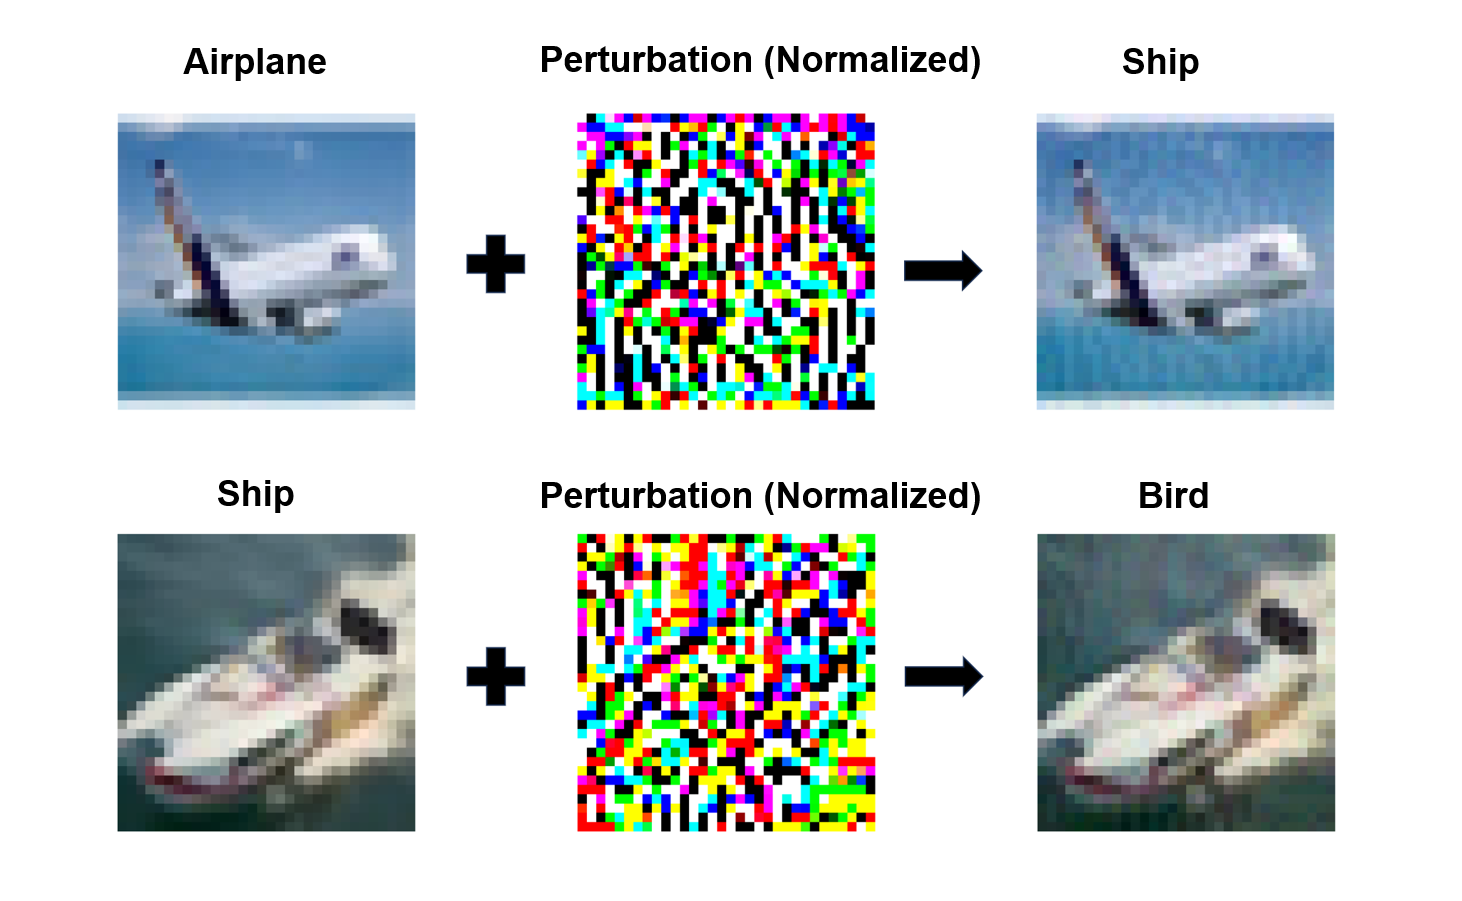
\includegraphics[width=0.85\linewidth]{images/Adversarial examples.png}
    \caption{Adversarial examples on CIFAR-10. Each row shows the original image with true label(left), the perturbation (middle), and the adversarial image with isclassification (right).}

    \label{fig:adv_examples}
\end{figure}

To address these threats, a wide range of adversarial defense strategies have been proposed. A comprehensive systematization of certified robustness techniques was provided by Li et al.~\cite{li2023sok}, who categorized existing methods into verification-based approaches (e.g., LP~\cite{wong2018provable} and MILP~\cite{tjeng2017evaluating}) and training-based approaches (e.g., robust training with bound propagation~\cite{gowal2018effectiveness}). This work also highlights the trade-offs between the quality of computed certified bounds and scalability. 
Certified defenses~\cite{cohen2019certified, gowal2018effectiveness} provide provable guarantees against norm-bounded attacks (e.g., $\ell_\infty$), but often suffer from scalability and computational cost. In contrast, empirical defenses, such as adversarial training~\cite{madry2017towards, wong2020fast} are more scalable and effective in practice but can remain susceptible to adaptive or unforeseen attacks~\cite{tramer2020adaptive}.


This project builds on both certified and empirical perspectives. In particular, we investigate certified training methods such as the LP-based training proposed by Wong and Kolter~\cite{wong2018provable}, alongside empirical defenses.

Among empirical approaches, ensemble-based defenses have emerged as a promising direction for enhancing robustness. By aggregating predictions from multiple models, ensembles can potentially mitigate the vulnerabilities of individual models and improve overall reliability~\cite{abbasi2017robustness, pang2019improving}. Traditional ensemble methods, such as majority voting or logits averaging, have shown some improvement in robustness, but they often lack a principled way to assess prediction confidence, making it difficult to determine whether the ensemble’s output is reliable under adversarial conditions.


Recently, \textit{CrossMax} was introduced as part of the ``Ensemble Everything Everywhere'' framework~\cite{fort2024ensemble}, providing a robust aggregation mechanism for ensemble predictions. We expand on the original design: Traditional ensemble methods, such as averaging logits or probabilities, are susceptible to attacks targeting a single model, where an outlier prediction can dominate the aggregate output. CrossMax mitigates this by drawing inspiration from Vickrey auctions: it considers each model as a bidder and aggregates predictions using the $k$-th largest logits per class rather than the maximum. Additional normalization steps, including subtracting each predictor's maximum and the per-class maximum, prevent individual models or classes from dominating spuriously. This dynamic aggregation ensures that the ensemble's decision reflects consistent agreement across models, enhancing robustness against targeted adversarial perturbations.


However, subsequent work~\cite{zhang2024evaluating} challenged these findings, attributing the apparent robustness gains largely to \textit{gradient masking}, a known evaluation pitfall. They showed that attacking the \textit{mean aggregation} mechanism and evaluating CrossMax yields stronger adversarial examples than directly attacking CrossMax itself, suggesting that CrossMax impedes gradient-based optimization rather than offering true robustness improvements.


Despite this criticism, CrossMax retains robustness benefits by leveraging model disagreement. Prior works focused solely on \textit{single-label predictions}. In contrast, we highlight a novel property: \textbf{CrossMax can produce multi-label prediction sets with a bounded size}, as detailed in Appendix~\ref{appendix:crossmax-bound}. The proportion of samples with single-label predictions, i.e., prediction sets of size one, serves as a proxy for ensemble confidence under attack. Our experiments reveal that ensembles of robustly trained models maintain a more stable single-label prediction rate compared to naturally trained ones, offering a new perspective on interpreting ensemble confidence and robustness beyond standard accuracy metrics.


The contributions of this work are threefold. First, we provide a comprehensive empirical evaluation of ensemble defense methods against strong white-box adversarial attacks, including APGD, FABAttack\_PT, and targeted APGD, as well as the query-based black-box SquareAttack~\cite{croce2020reliable}, highlighting their robustness performance under varying perturbation budgets. Second, we systematically study the effects of architectural diversity and training perturbation budgets on ensemble robustness, revealing important trade-offs and insights. Third, we analyze ensemble confidence behaviors across multiple aggregation strategies, with a particular focus on CrossMax, elucidating its strengths as well as limitations in practical robustness scenarios.

Through these contributions, we offer new insights into how ensemble methods, especially CrossMax, can effectively bridge the gap between certified robustness guarantees and empirical adversarial resilience, balancing robustness with clean accuracy. The code and implementation details for this project are available at our GitHub repository: https://github.com/samavi/lpsdp.git

% ----------------- CHAPTER 2 -----------------
\chapter{Literature Review}

\section{Empirical Adversarial Defenses}
\indent

Empirical adversarial defenses aim to improve robustness by training models directly on adversarially perturbed inputs. While adversarial training has proven highly effective in practice, its robustness is inherently bounded by the strength and diversity of attacks used during training, and models often remain vulnerable to unseen or stronger adversaries.

One of the most widely adopted techniques is \textit{adversarial training}, introduced by Madry et al.~\cite{madry2017towards}, which frames robustness as a min-max optimization problem. In this formulation, the model is trained on adversarial examples crafted using Projected Gradient Descent (PGD), making it robust against a strong first-order adversary. This approach has become a de facto standard for empirical robustness due to its effectiveness across various datasets and architectures.

Several improvements to adversarial training have since been proposed. For instance, TRADES~\cite{zhang2019theoretically} introduces a regularization term to explicitly control the trade-off between clean accuracy and adversarial robustness. MART~\cite{wang2019improving} emphasizes misclassified examples during training to improve robustness further. These methods demonstrate that empirical robustness can be systematically enhanced through better loss design and training strategies.

Despite their success, empirical methods face several limitations. First, they offer no formal guarantees: robustness is only evaluated against specific attacks used during training and testing. As a result, these defenses can remain vulnerable to stronger or adaptive attacks~\cite{tramer2020adaptive}. Second, adversarial training often incurs substantial computational cost and can lead to drops in clean accuracy~\cite{rice2020overfitting}. Moreover, empirical defenses tend to be sensitive to hyperparameter choices and may not generalize well across different threat models or perturbation budgets.

Nonetheless, empirical defenses remain a practical choice for real-world deployment due to their scalability and relatively high robustness under standard evaluations. However, adversarial training often requires substantial computational resources and may not generalize well across unseen attack patterns. In contrast, our study explores an alternative path to robustness by investigating the behavior of naturally trained models and their ensembles under strong adversarial attacks. Rather than relying on specialized training procedures, we focus on how ensemble diversity and score-level aggregation can contribute to adversarial robustness, offering a complementary perspective to conventional empirical defenses.


\section{Provable Adversarial Defenses}

\indent

Empirical adversarial defenses, such as adversarial training~\cite{madry2017towards}, improve robustness by exposing models to adversarial examples generated through specific attack algorithms. Provable defenses~\cite{wong2018provable, cohen2019certified} aim to offer formal guarantees that a model's prediction remains unchanged under all perturbations within a specified norm-bound (e.g., $\ell_\infty$ or $\ell_2$ balls), constructing mathematical certificates of robustness to ensure resilience against any perturbation within the threat model.

Within the landscape of certified robustness, existing approaches can be broadly categorized into complete, incomplete relaxation-based, and probabilistic approaches. Complete methods provide exact guarantees but rarely scale beyond small networks, while incomplete methods trade off exactness for tractability, and probabilistic approaches certify robustness in expectation under random noise distributions.


Complete methods aim to exhaustively verify the robustness of neural networks by exploring the entire input space within a perturbation set. Mixed-Integer Linear Programming (MILP) is one representative approach, where adversarial robustness is encoded as a set of linear constraints with integer variables for ReLU activations~\cite{tjeng2017evaluating}. Other complete verification techniques include satisfiability modulo theory (SMT)-based solvers~\cite{ehlers2017formal}, which encode network decisions into logical constraints, and Reluplex~\cite{katz2017reluplex}, an extension of the Simplex algorithm tailored to piecewise-linear activations. More recently and branch-and-bound frameworks~\cite{bunel2018unified} combine symbolic propagation with search to improve scalability. Despite their theoretical appeal and ability to provide exact robustness guarantees, these methods suffer from severe computational complexity, restricting their applicability to small networks or shallow architectures. Consequently, complete methods are often viewed as valuable for benchmarking and understanding robustness, but impractical for large-scale deployment.

In contrast, incomplete methods such as Linear Programming (LP)-based methods introduced by Wong and Kolter~\cite{wong2018provable} offer a more scalable alternative by relaxing the ReLU nonlinearity using convex outer approximations. By enabling efficient bound propagation through the network, this relaxation allows robustness training and certification to scale to larger models. The core idea in LP-based training is to optimize a convex upper bound on the worst-case loss within the perturbation set. At training time, models are encouraged to give correct prediction even under all adversarial perturbations. While this method provides certified robustness during training, it introduces a trade-off: increasing the tightness of the convex bounds typically reduces clean accuracy, since the additional constraints restrict the model’s capacity to fit clean data. Moreover, achieving tighter relaxations requires solving more complex optimization problems, which significantly limits scalability to deeper or more complex architectures. To obtain even lower certified bounds on adversarial loss, another incomplete approach within certified robustness employs semidefinite programming (SDP). In particular, Raghunathan et al.~\cite{raghunathan2018semidefinite} proposed an SDP-based relaxation to certify the robustness of ReLU networks. By formulating the adversarial perturbation problem as a quadratic program over the input, the authors derived an SDP relaxation that provides tighter certified bounds on adversarial loss than linear methods (e.g., LP), especially for small networks. However, due to the high computational cost of SDP solvers, these methods do not scale well to larger architectures or datasets. This trade-off between tightness and scalability remains a key challenge in certified robustness. To improve efficiency at the cost of looser certificates, Interval Bound Propagation (IBP)~\cite{gowal2018effectiveness} propagates input intervals through the network to estimate bounds on output perturbations. Though IBP is significantly more scalable, its bounds are often too loose to guarantee robustness in challenging scenarios. More recent work has attempted to combine the advantages of LP and IBP to balance tightness and computational efficiency~\cite{zhang2019towards}. In this project, we select LP-based certified training as the representative method because it offers a practical balance between rigor and scalability. Compared to more computationally expensive approaches such as SDP, LP certification can be applied at reasonable cost to non-trivial architectures on CIFAR-10, where it has already been successfully demonstrated~\cite{wong2018scaling}. This makes LP-based methods a widely adopted benchmark in certified robustness research and a suitable choice for our comparative study of ensembles, where both clean accuracy and robustness must be jointly examined.


Other approaches, such as randomized smoothing~\cite{cohen2019certified}, offer probabilistic robustness guarantees by averaging predictions over random noise injections. One key advantage is that randomized smoothing is architecture-agnostic and scales effectively to large datasets such as ImageNet, without requiring modifications to the underlying model. It is also simple to implement, since it only requires injecting noise during training and inference. Moreover, unlike purely empirical defenses, randomized smoothing provides certified guarantees in a probabilistic sense, which makes it an attractive practical compromise between scalability and formal robustness. However, its guarantees are typically restricted to $\ell_2$-norm perturbations and inference requires many stochastic forward passes, which can increase computational cost.

Despite their theoretical appeal, provable defenses remain constrained in practice. They often struggle to scale to large datasets like ImageNet or architectures with high capacity. Moreover, many provable training methods (e.g., LP-based or IBP-based) suffer from loose bounds when facing higher threat perturbation budgets, especially in high-dimensional input spaces.


In our study, we use LP-based convex relaxation as a certified robustness method. We adopt the convex relaxation framework introduced by Wong and Kolter~\cite{wong2018provable} to train robust base models, which are then integrated into ensemble systems. This allows us to investigate how certified training contributes to ensemble-level robustness, and whether ensembles of provably robust models retain their guarantees or exhibit new emergent behavior when combined under ensemble mechanisms like CrossMax~\cite{fort2024ensemble}.




\section{Ensemble Methods for Robustness}
\indent

Ensemble learning is a widely adopted technique in machine learning to enhance generalization by aggregating predictions from multiple models. In adversarial settings, ensembles can provide improved robustness by diversifying model behaviors, making it more difficult for a single perturbation to simultaneously fool all models. Classical ensemble strategies include majority voting and soft (logit) averaging, both of which have been investigated in adversarial contexts.

Tramèr et al.~\cite{tramer2017ensemble} systematically analyzed ensemble adversarial training, showing that ensembles of independently trained models can offer improved robustness. However, they also revealed that shared vulnerabilities among ensemble members can lead to a lack of diversity, making the ensemble susceptible to adaptive attacks. Strauss et al.~\cite{strauss2017ensemble} compared simple ensemble aggregation methods and observed that improvements under white-box attacks were marginal unless model diversity was explicitly enforced.

To address the lack of diversity in models, later works proposed diversity-promoting training objectives. Pang et al.~\cite{pang2019improving} introduced adversarially robust ensembles by maximizing disagreement among member models under clean and adversarial inputs. Similarly, Kariyappa and Qureshi~\cite{kariyappa2019improving} enforced orthogonality in input gradients across models to encourage diverse local decision boundaries. These methods reflect a growing awareness that ensemble effectiveness under adversarial threat relies not just on the number of models, but on the diversity and independence of their decision-making processes.

However, while some recent works have explored certified robustness in ensembles through training-time strategies, such as weighted optimization~\cite{zhang2019enhancing} or diversity regularization~\cite{yang2021certified}, the use of certified training methods such as LP-based approaches~\cite{wong2018provable} remains underexplored in the ensemble setting. In particular, there is limited investigation into purely inference-time ensemble aggregation for certified robustness, which motivates our study.

\textit{CrossMax}, introduced in the ``Ensemble Everything Everywhere'' framework~\cite{fort2024ensemble}, presents a novel aggregation strategy inspired by Vickrey auctions~\cite{vickrey1961counterspeculation}. It dynamically selects logits from intermediate layers based on cross-layer agreement, aiming to improve robustness through feature-level diversity. While originally applied to self-ensembling within a single model, its core idea naturally extends to ensembles composed of structurally different models, where architectural heterogeneity may offer further benefits. Later analysis by Zhang et al.~\cite{zhang2024evaluating} raised concerns about the robustness claims made in the original work, pointing to gradient masking as a potential confounding factor. Their findings highlighted the need for more rigorous evaluation.

Motivated by these insights, we extend CrossMax to a multi-model setting, where constituent networks differ in both architecture and training regime. This shift from the original self-ensemble design leverages model-level diversity to enhance robustness. Furthermore, in response to the concerns raised by~\cite{zhang2024evaluating} regarding potential gradient masking, we employ stronger, attack-aware evaluation protocols to ensure that any observed robustness gains cannot be attributed to such artifacts. While the robustness of CrossMax remains debated, its reliance on cross-model agreement makes it a candidate for further exploration in ensemble contexts. In this work, we extend CrossMax beyond self-ensembling and apply it across ensembles of independently trained models.




\section{Confidence and Robustness}
\indent

Recent advances in adversarial robustness have increasingly recognized the importance of not only achieving high accuracy but also reliably assessing the confidence of model predictions under adversarial perturbations. Confidence-aware methods seek to utilize uncertainty or disagreement signals within model predictions to better detect adversarial examples or to estimate prediction reliability~\cite{gal2016dropout}.

In the context of ensemble methods, confidence evaluation often involves analyzing inter-model agreement or prediction consistency as a proxy for robustness. Traditional ensemble aggregation techniques, such as majority voting or logits averaging, do not explicitly capture these uncertainty characteristics. To address this gap, novel approaches have been proposed to leverage intra-ensemble dynamics and disagreement patterns to infer adversarial risk~\cite{pang2019improving, abbasi2017robustness}.

In our study, we adapt CrossMax to a more general ensemble setting by applying it across a pool of independently trained models, rather than within a single network. Our adaptation of CrossMax allows it to act as a voting mechanism over logits selected from different independently trained models. Notably, this often results in not only a single predicted label but sometimes a \textit{prediction set} containing multiple plausible classes. This behavior was not discussed in the original CrossMax paper, but we find it particularly informative under adversarial conditions.

We define the prediction confidence of CrossMax as the proportion of samples for which it yields a unique prediction. Rather than interpreting higher singleton prediction rates as inherently better, we emphasize the stability of this confidence signal under adversarial perturbations. This insight introduces a novel perspective on ensemble confidence, where prediction set structure, rather than just softmax scores, serves as an interpretable, robust indicator of model reliability. Such confidence-aware outputs offer potential utility in downstream tasks such as adversarial example detection or adaptive defense triggering.
% ----------------- CHAPTER 3 -----------------
\chapter{Comparative Study Design}

\section{Study Objectives and Comparative Approach}
\indent

This chapter presents the design of a comparative study between \textit{LP certified models} and \textit{standard non-certified models}, both in their individual form and as ensembles. The goal is to evaluate the impact of certified training on robustness, prediction diversity and confidence estimation under adversarial settings.

We select \textit{LP certification} as the representative certified defense, since it provides \emph{provable robustness guarantees} against $L_\infty$-bounded perturbations by formulating the verification of adversarial robustness as a linear optimization problem. Compared to heuristic empirical defenses, LP-based certification is both mathematically rigorous and practically effective on moderate-scale datasets such as CIFAR-10, making it a widely adopted benchmark in robustness research.

All robustness training and adversarial perturbations considered in this study are constrained under the $L_\infty$ norm:
\[
\|\delta\|_\infty \leq \epsilon,
\]
which aligns with the perturbation model used in the LP certification framework and is widely adopted in adversarial robustness research for its interpretability and practical relevance in image domains.




The study focuses on four configurations:
\begin{itemize}
    \item Single standard model (non-certified), representing typical training without explicit robustness guarantees.
    \item Single LP-trained model, where robustness guarantees are provided via convex relaxations during training.
    \item Standard ensemble model, aggregating multiple independently trained standard models to explore diversity benefits.
    \item LP-trained ensemble model, aggregating multiple certified models to investigate the interplay between certification and ensembling.
\end{itemize}

The comparison is performed on the CIFAR-10 dataset~\cite{krizhevsky2009learning}, ensuring consistent model architectures across LP and standard variants to isolate the effect of certified training. Evaluations are conducted across multiple perturbation strengths to capture robustness trends at varying threat levels.

For ensemble methods, beyond robustness accuracy and diversity, we also assess the prediction confidence by measuring the proportion of single-label outputs produced by the CrossMax aggregation method compared to ambiguous multi-label outputs (details in Section~\ref{sec:evaluation dimensions}). This metric serves as a novel confidence-related indicator, potentially reflecting ensemble certainty under adversarial perturbations.

The approach is motivated by two main \textbf{objectives}:
\begin{itemize}

    \item To understand how certified robustness properties at the networks  level in the ensemble propagate or improve when models are combined into ensembles.
    \item To investigate whether confidence-related signals emerging from advanced aggregation strategies like CrossMax can provide complementary robustness insights beyond robust accuracy.
\end{itemize}

Together, these analyses aim to deepen understanding of the trade-offs and synergies between certification, ensembling, and confidence estimation in the pursuit of more reliable adversarial defenses.

\section{Evaluation Dimensions and Formal Definition}
\label{sec:evaluation dimensions}
\indent


To ensure clarity and reproducibility, we define the evaluation dimensions as follows:

\subsection{Robustness Accuracy}
\indent

In adversarial machine learning, robustness quantifies a model's ability to maintain correct predictions under bounded perturbations of the input.  
Following the formalism of \cite{kielhofer2025robustness}, we adopt the $\ell_\infty$ norm as the perturbation metric throughout this work.  
For a perturbation size $\epsilon$, robust accuracy can be formally defined as follows:

\begin{definition}[Robust accuracy]
Consider a neural network $f:\mathbb{R}^n \to \mathbb{N}$ and a perturbation size $\epsilon$. 
Robust accuracy indicates the probability that the network is $\epsilon$-robust for an arbitrary classified reference input $x_0$. 
This is denoted as
\begin{equation}
P(\epsilon) := P\left(\{x_0 : \|x - x_0\| < \epsilon \Rightarrow f(x) = y_{x_0}\}\right).
\end{equation}
\end{definition}

\begin{definition}[Estimator of robust accuracy]
Given a test set $D$ that was not used for training, an estimator for robust accuracy is obtained by
\begin{equation}
P_D(\epsilon) := \frac{|\{x_0 \in D : \forall x \in \mathbb{R}^n,\ \|x - x_0\| < \epsilon \Rightarrow f(x) = y_{x_0}\}|}{|D|}.
\end{equation}
\end{definition}


Following \cite{kielhofer2025robustness}, we rigorously distinguish between two related but distinct metrics:  
\emph{empirical robust accuracy}, measured under adaptive adversarial attacks such as PGD or AutoAttack; and  
\emph{certified robust accuracy}, computed via linear LP verification~\cite{wong2018provable,gowal2018effectiveness} to provide a guaranteed lower bound within a specified perturbation budget.  
This deliberate distinction avoids ambiguity with alternative terms (e.g., astuteness or adversarial accuracy) and enables direct comparison between attack-based evaluation and formally verified guarantees. \textbf{In the following content, all experimental robust accuracy refers to estimator of robust accuracy, and certified robust accuracy will be specifically indicated.}

\subsection{Ensemble Diversity and Confidence Measures}
\label{sec:diversity-confidence}

\indent

To analyze the relationship between ensemble diversity, confidence, and robustness, we evaluate five complementary metrics:
\emph{(1) prediction diversity}, 
\emph{(2) softmax confidence}, 
\emph{(3) prediction entropy}, 
\emph{(4) mutual information (MI)}, 
and \emph{(5) CrossMax Confidence}(details in Section~\ref{sec:crossmax confidence}).
These measures are computed on both clean and adversarial examples, enabling a quantitative comparison of their behaviors under distributional shifts.

The use of prediction diversity as a robustness metric builds upon prior work, such as Pang et al.~\cite{pang2019improving}, who introduce diversity among non-maximal predictions to improve ensemble adversarial robustness, and Abbasi et al.~\cite{abbasi2020toward}, who demonstrate the utility of diversity in detecting adversarial samples. On the other hand, mutual information (MI) as a tool to characterize model uncertainty under attack has been explored by Zhou et al.~\cite{zhou2022improving}, providing insight into changes in model confidence. The broader theoretical relationship between ensemble diversity, robust accuracy, and deception resilience is comprehensively discussed in Liu et al.~\cite{liu2019deep}, offering foundational support for our multi-metric evaluation framework. Here are the exact definition of those metrics mentioned above in our experiments:


\paragraph{Prediction Diversity}
For an ensemble of $M$ classifiers $\{f_{\theta_m}\}_{m=1}^M$, prediction diversity quantifies the pairwise disagreement rate:
\begin{equation}
\text{Div} = \frac{1}{M(M-1)} \sum_{1 \leq i \neq j \leq M} 
\mathbb{P}\big( f_{\theta_i}(x) \neq f_{\theta_j}(x) \big).
\end{equation}

where $\mathbb{P}$ denotes the empirical probability over the input distribution (e.g., the test set).
A higher value indicates greater heterogeneity among ensemble members, 
i.e., larger diversity in their learned decision boundaries and predictive behaviors. 
Such diversity reduces the chance that a single adversarial perturbation can simultaneously fool all models, 
thereby improving robustness against transferable adversarial examples.
However, excessive diversity may harm clean accuracy if individual models disagree too often on clean inputs.

\paragraph{Softmax Confidence}
Similar to the definition in~\cite{guo2017calibration}, 
for a single model $f_{\theta_m}$ producing logits 
$\mathbf{z}^{(m)}(x) = (z^{(m)}_0(x), \ldots, z^{(m)}_{K-1}(x))$ 
over $K$ classes, the single-model softmax confidence is defined as the maximum softmax probability:

\begin{equation}
\text{Conf}_{\mathrm{Soft}}^{(m)}(x) 
= \max_{c \in \{0, \ldots, K-1\}} 
\frac{\exp(z_c^{(m)}(x))}{\sum_{j=0}^{K-1} \exp(z_j^{(m)}(x))}.
\label{eq:soft_conf_single}
\end{equation}

For an ensemble with $M$ members, we define the ensemble softmax confidence as the member-wise average of the single-model confidences:

\begin{equation}
\overline{\text{Conf}}_{\mathrm{Soft}}(x) 
= \frac{1}{M} \sum_{m=1}^{M} \text{Conf}_{\mathrm{Soft}}^{(m)}(x),
\label{eq:soft_conf_ensemble}
\end{equation}

\noindent which reflects the average confidence across all models, without first combining logits.



This reflects the aggregate confidence across models, 
while disregarding potential disagreement among individual members.
Note that this differs from computing the maximum probability after ensemble averaging, 
and is chosen here to explicitly capture individual member confidence.

\paragraph{Prediction Entropy}
Prediction entropy measures the uncertainty of the ensemble’s averaged softmax output:
\begin{equation}
H(x) = - \sum_{k=1}^K p_k(x) \log p_k(x),
\quad
p_k(x) = \frac{1}{M} \sum_{m=1}^M \sigma_k(\mathbf{z}_m(x)).
\end{equation}
where $\sigma_k(\cdot)$ denotes the softmax probability assigned to class $k$ by a model, 
and $p_k(x)$ is the ensemble-averaged predictive probability for class $k$.
A higher entropy value indicates greater predictive uncertainty and weaker class separation, 
while a lower entropy suggests stronger consensus and more confident predictions across the ensemble~\cite{liu2019deep}.

\paragraph{Mutual Information (MI)}
Mutual Information, motivated by Bayesian ensemble theory, decomposes predictive uncertainty into two components: 
\emph{aleatoric uncertainty} (inherent data noise that cannot be reduced) and 
\emph{epistemic uncertainty} (uncertainty due to limited model knowledge). 
Formally, it is defined as
\begin{equation}
\text{MI}(x) = H(x) - \frac{1}{M} \sum_{m=1}^M H_m(x),
\end{equation}

where $H(x)$ is the total predictive entropy as defined above, and

\begin{equation}
H_m(x) = - \sum_{k=1}^K \sigma_k(\mathbf{z}_m(x)) \log \sigma_k(\mathbf{z}_m(x))
\end{equation}

is the entropy of the $m$-th model’s predictive distribution.
A higher MI indicates greater disagreement among models, thereby capturing epistemic uncertainty.




\section{LP Models and Dataset Setting}
\label{sec:methodology-models}
\indent

Following the setup in \cite{wong2018scaling}, we adopt the CIFAR-10 dataset for all experiments. 
The LP-trained models are obtained from the authors’ released pre-trained checkpoints, covering three architectures:
\begin{itemize}
    \item \textbf{Small}: 2 convolutional layers (16, 32 filters) and 1 fully connected layer (100 units).
    \item \textbf{Large}: 4 convolutional layers (32, 32, 64, 64 filters) and 2 fully connected layers (512 units).
    \item \textbf{ResNet}: 4 residual blocks (16, 16, 32, 64 filters) following \cite{zagoruyko2016wide}.
\end{itemize}
For each architecture, two LP-trained versions are available:
\begin{itemize}
    \item $\epsilon=2.0/255$ (denoted \textbf{2px} in the following content)
    \item $\epsilon=8.0/255$ (denoted \textbf{8px} in the following content)
\end{itemize}

\begin{table}[h]
\centering
\caption{Certified robust and clean accuracy of LP-trained on CIFAR-10 test set at different perturbation budgets.  
Certified robust accuracy values are reported at each model’s certified perturbation level.}
\label{tab:lp_cert_acc_detailed}
\begin{tabular}{lccc}
\toprule
\textbf{Model} & \textbf{Eps.} & \textbf{CRA (\%)} & \textbf{Clean Acc. (\%)} \\
\midrule
Small   & $2/255$ & 46.41 & 60.86 \\
Large   & $2/255$ & 52.59 & 67.71 \\
ResNet  & $2/255$ & 51.52 & 66.33 \\
Small   & $8/255$ & 20.54 & 27.60 \\
Large   & $8/255$ & 16.03 & 19.01 \\
ResNet  & $8/255$ & 21.50 & 27.05 \\
\bottomrule
\end{tabular}
\end{table}


\section{Ensemble Methods}
\indent

We focus on three aggregation rules due to their representativeness and contrastive nature. Majority Voting~\cite{dietterich2000ensemble} serves as the classical baseline, Logits Averaging~\cite{lakshminarayanan2017simple} captures probabilistic information from individual models, and CrossMax~\cite{fort2024ensemble} represents a robustness-oriented approach that we aim to investigate. This selection allows us to compare traditional ensemble strategies with our proposed method under a unified framework.

\subsection{Majority Voting}  
Given a set of $M$ base models, each producing a predicted class label $\hat{y}_m$ for an input, the Majority Voting ensemble outputs the class with the highest frequency among these predictions:
\begin{equation}
    \hat{y}_{\small{MV}} = \arg\max_{c \in \mathcal{Y}} \sum_{m=1}^M \mathbb{I}(\hat{y}_m = c),
\end{equation}
where $\mathbb{I}(\cdot)$ is the indicator function.

\noindent
\textbf{Limitation.}  
When facing an adaptive adversary, the attacker does not necessarily need to fool all the networks inside the ensemble model simultaneously.
Instead, it is sufficient to target a majority subset of comparatively ``weaker'' models whose decisions dominate the vote.
This makes Majority Voting potentially vulnerable if the ensemble contains several models with similar failure modes.

\subsection{Logits Averaging}  
Each base model outputs a logit vector $\mathbf{z}_m = (z_{m,1}, \dots, z_{m,c}) \in \mathbb{R}^C$, 
where $z_{m,c}$ denotes the logit for class $c$.  
The ensemble average logit vector is computed as
\begin{equation}
    \bar{\mathbf{z}} = \frac{1}{M} \sum_{m=1}^M \mathbf{z}_m,
\end{equation}
whose $c$-th component is $\bar{z}_c = \frac{1}{M}\sum_{m=1}^N z_{m,c}$. 
The final prediction is then obtained as
\begin{equation}
    \hat{y}_{\text{LA}} = \arg\max_{c \in \mathcal{Y}} \bar{z}_c.
\end{equation}


\noindent
\textbf{Limitation.}  
Because the magnitude of logits can vary significantly across models, some models may exert disproportionately large influence on the averaged logits.
An adversary can exploit this by preferentially attacking such ``high-impact'' models, shifting the ensemble decision even without altering the outputs of the other members.


\subsection{CrossMax}
\label{sec:crossmax}
\indent

We now present the CrossMax aggregation rule, designed to mitigate both predictor dominance (one model overwhelmingly influencing the final decision) and class dominance (one class consistently winning regardless of model variation). Let 
\[
\mathbf{Z} \in \mathbb{R}^{M \times C}
\]
denote the logits matrix, where $M$ is the number of predictors and $C$ is the number of classes. The $i$-th row $\mathbf{z}_i$ corresponds to the logits from the $i$-th predictor.

The algorithm of the original CrossMax method proposed by Fort and Lakshminarayanan~\cite{fort2024ensemble} is in Appendix~\ref{alg:crossmax}.  
In our work, we have extended this approach by introducing two additional post-processing strategies to handle ambiguous predictions where multiple classes share the $k$-th largest logit value.  
Here are the detailed process and two strategies:



\paragraph{Step 1: Removing predictor dominance.}  
For each predictor $i$, we normalize its logits vector $\mathbf{z}_i$ by subtracting its maximum value:
\[
\tilde{\mathbf{z}}_i = \mathbf{z}_i - \max_{c} \mathbf{z}_{i,c}.
\]
This ensures that no single predictor's scale or offset can disproportionately affect the aggregation.

\paragraph{Step 2: Removing class dominance.}  
We normalize each column (class) across all predictors by subtracting the maximum over predictors:
\[
\hat{\mathbf{z}}_{i,c} = \tilde{\mathbf{z}}_{i,c} - \max_{j} \tilde{\mathbf{z}}_{j,c}.
\]
This removes the bias where certain classes might consistently have higher raw logits across predictors.

\paragraph{Step 3: $k$-th max aggregation.}  
After both normalizations, the CrossMax rule computes the $k$-th largest value across predictors for each class:
\[
s_c = \operatorname{k\text{-}max}_{i} \ \hat{\mathbf{z}}_{i,c}.
\]
The final predicted class is
\[
\hat{y} = \arg\max_{c} s_c.
\]
Here, $k$ is a tunable hyperparameter that controls the balance between robustness and sensitivity: $k=1$ reduces to the classical max rule (most aggressive selection), larger $k$ values give more weight to consensus among predictors.

\paragraph{Ambiguous versus Exact Prediction:}
When computing the $k$-th largest value per class, ties may occur:
\begin{itemize}
    \item \emph{Ambiguous prediction:} All classes sharing the $k$-th largest value are retained as possible outputs.
    \item \emph{Exact prediction:} If multiple classes tie for the $k$-th largest value, we break the tie as follows:
    \begin{enumerate}
        \item Randomly select $M' \in \{5,4,3\}$ predictors from the $M=6$ base models.
        \item Re-run CrossMax on the selected subset to obtain a predicted class.
        \item Repeat the above until $M'$ predictions are collected.
        \item Apply majority voting on the resulting $M=6$ predictions to obtain the final output.
    \end{enumerate}
\end{itemize}
This two-level selection scheme balances robustness against adversarial perturbations with the need for a deterministic final prediction.  
As proved in Appendix~\ref{appendix:crossmax-bound}, the maximum size of such ambiguous prediction sets is inherently limited by the number of base models and the choice of $k$ and $M$.

\begin{table}[h]
\centering
\caption{Example of logits aggregation for a single input across different ensemble methods under an adversarial perturbation (target class = 0).}
\label{tab:ensemble_example}
\renewcommand{\arraystretch}{1.2}
\small
\begin{tabular}{lcccccccccc}
\toprule
\textbf{Model/Method} & \multicolumn{10}{c}{\textbf{Logits per Class}} \\
\cmidrule(lr){2-11}
 & 0 & 1 & 2 & 3 & 4 & 5 & 6 & 7 & 8 & 9 \\
\midrule
ResNet\_8px   & 0.949 & 0.645 & -0.302 & -0.599 & -0.781 & -0.658 & -1.470 & -0.339 & \underline{\textbf{1.526}} & 1.029 \\
ResNet\_2px   & \underline{\textbf{4.712}} & -0.705 & 1.831 & -1.449 & 1.285 & -2.892 & -3.150 & -1.248 & 2.965 & -1.350 \\
Large\_8px    & 1.003 & 0.173 & -0.186 & -0.500 & -0.671 & -0.779 & -0.867 & 0.109 & \underline{\textbf{1.026}} & 0.691 \\
Large\_2px    & \underline{\textbf{5.777}} & -0.457 & 1.798 & -1.821 & 0.262 & -2.488 & -2.819 & -1.751 & 2.907 & -1.407 \\
Small\_8px    & 1.609 & 0.423 & 0.085 & -0.515 & -0.545 & -0.727 & -1.784 & -0.729 & \underline{\textbf{1.767}} & 0.414 \\
Small\_2px    & 2.880 & -0.929 & 1.646 & -1.195 & 1.370 & -1.808 & -2.957 & -0.931 & \underline{\textbf{3.246}} & -1.323 \\
\midrule
\textit{Logits Averaging} & \underline{\textbf{2.822}} & -0.142 & 0.979 & -1.013 & 0.153 & -1.892 & -2.341 & -0.815 & 2.240 & -0.658 \\
\textit{Majority Voting}  & 2 & 0 & 0 & 0 & 0 & 0 & 0 & 0 & \underline{\textbf{4}} & 0 \\
\textit{CrossMax}         & \underline{\textbf{0.000}} & -0.029 & -0.388 & -0.599 & -0.179 & -0.379 & -1.103 & -0.949 & \underline{\textbf{0.000}} & -0.163 \\
\bottomrule
\end{tabular}

\vspace{0.5em}
\footnotesize
\raggedright
\textbf{Note:} This example corresponds to an adversarially perturbed input targeting class~0. 
Under this setting, CrossMax produces a prediction set rather than a single label. 
For the \textit{ambiguous} variant, the prediction set is $\{0, 8\}$, reflecting two equally plausible classes after aggregation. 
For the \textit{exact} variant, only class~0 is retained in the prediction set. 
In contrast, logits averaging selects class~0 as the top-1 prediction, while majority voting predicts class~8 due to the highest vote count.
\end{table}


\paragraph{CrossMax Confidence}
\label{sec:crossmax confidence}
We evaluate the \emph{CrossMax Confidence} of the ensemble, which quantifies the proportion of test inputs for which the CrossMax-Ambiguous set contains exactly one label.  
Formally, if $\mathcal{A}(x)$ denotes the prediction set produced by CrossMax-Ambiguous for input $x$, the CrossMax Confidence is defined as:
\[
\text{Conf}_{\text{CrossMax}} = \frac{1}{|\mathcal{D}_{\text{test}}|} \sum_{x \in \mathcal{D}_{\text{test}}} \mathbb{I}\left[|\mathcal{A}(x)| = 1\right],
\]
where $\mathbb{I}[\cdot]$ is the indicator function and $\mathcal{D}_{\text{test}}$ denotes the test dataset.
A high CrossMax Confidence indicates that the ensemble, under the CrossMax aggregation, produces an unambiguous decision for most inputs, while a lower value suggests increased prediction set size and hence greater ambiguity.



\section{Fair Comparison Protocol}
\indent

To ensure that the comparative analysis between LP-based ensembles and standard ensembles is both fair and reproducible, a rigorous evaluation protocol is followed. This protocol is designed to eliminate potential confounding factors that could bias the results, allowing any observed differences to be attributed solely to the ensemble strategy under investigation. The key principles are as follows:

\begin{itemize}
    \item \textbf{Identical Dataset:} All evaluations are conducted on the CIFAR-10 test set, which consists of 10,000 fixed images. The same set of images is used across all models and experiments to prevent variability arising from data selection.
    
    \item \textbf{Matched Architectures:} For every LP-trained model, there exists a corresponding standard model with the exact same architecture (e.g., ResNet, Large, Small variants). This ensures that any performance difference is not due to architectural capacity or depth.
    
    \item \textbf{Equal Ensemble Size:} Both LP and standard ensembles are composed of exactly six networks inside ensemble models. This parity prevents the ensemble size from acting as a confounding variable, thereby isolating the effect of the training paradigm and aggregation strategy.
    
    \item \textbf{Consistent Training Data:} All models, whether LP or standard, are trained on the same CIFAR-10 training set, without differences in data preprocessing or augmentation. No additional data sources or synthetic examples are introduced, ensuring that the models' knowledge comes from an identical distribution.
    
    \item \textbf{Uniform Attack Protocol:} Adversarial robustness evaluation employs the same attack methods (specifically, AutoAttack) and identical perturbation budgets for all models. This guarantees that robustness measurements are directly comparable and unaffected by attack configuration biases.
    
    \item \textbf{Reproducibility and Random Seed Control:} All experiments are performed with fixed random seeds for data loading, model initialization, and attack generation. This minimizes stochastic variation in the results.
    
    \item \textbf{Identical Evaluation Metrics:} Performance is assessed using the same set of metrics: clean accuracy and adversarial accuracy, under identical evaluation conditions.
\end{itemize}
By adhering to this protocol, the comparative study ensures that the only variable under investigation is the ensemble composition and aggregation method, enabling a fair and unbiased evaluation of LP-based ensembles versus their standard counterparts.
% ----------------- CHAPTER 4 -----------------

\chapter{Experimental Evaluation}

\section{Experimental Setup}

\subsection{Dataset and Preprocessing}
\indent

All experiments are conducted on the CIFAR-10 dataset~\cite{krizhevsky2009learning}, which contains 50,000 training images and 10,000 testing images across 10 classes.
Images are first normalized to the range $[0,1]$. When applying adversarial perturbations, the perturbation budget $\epsilon$ is calculated relative to this scale, e.g., $2\text{px} = 2.0/255$ and $8\text{px} = 8.0/255$.
After perturbation, inputs are further normalized by subtracting the per-channel mean (0.485, 0.456, 0.406) and dividing by the per-channel standard deviation $0.225$. This normalization procedure aligns with the preprocessing used in \cite{wong2018scaling} for their LP-certified pre-trained models. It ensures consistent input distribution between standard and certified models.

\subsection{Standard Model Training}
\indent

We utilize three architectures previously described in Section~\ref{sec:methodology-models}: Small, Large, and ResNet.  
To provide a fair comparison with the LP-certified models, we train six standard (non-certified) models: two per architecture, using different checkpoints to increase ensemble diversity, as suggested in~\cite{fort2024ensemble}. The training procedure follows a standard supervised classification pipeline using cross-entropy loss and the Adam optimizer.  
Specifically, we train for 20 epochs with a learning rate of 0.001 and a batch size of 128, saving model checkpoints every 10 epochs to capture intermediate models.


\noindent


\begin{algorithm}[H]
\caption{Training and Evaluation Framework}
\label{alg:train_eval}
\begin{algorithmic}
\State \textbf{Require:} \\ Training data $\mathcal{D}_{\text{train}}$, test data $\mathcal{D}_{\text{test}}$, model $f_\theta$, learning rate $\eta$, number of epochs $T$, checkpoint interval $K$

\State \textbf{Training:} \\ Initialize model parameters $\theta$
\For{epoch $=1$ to $T$}
    \State Update $\theta$ by minimizing cross-entropy loss on $\mathcal{D}_{\text{train}}$ using Adam with step size $\eta$
    \State Evaluate current model on $\mathcal{D}_{\text{train}}$ and $\mathcal{D}_{\text{test}}$
    \If{$epoch \bmod K = 0$}
        \State Save model checkpoint with epoch identifier
    \EndIf
\EndFor
\Statex
\Function{Evaluate}{$f_\theta, \mathcal{D}$}
    \State Compute accuracy of $f_\theta$ on dataset $\mathcal{D}$ without parameter updates
\EndFunction
\end{algorithmic}
\end{algorithm}


The overall training and evaluation process is summarized in Algorithm~\ref{alg:train_eval}. During training, model parameters are updated epoch by epoch, and after each epoch we record both training and test accuracy to monitor convergence.  
To enable ensemble construction, we additionally save intermediate model checkpoints every $K=10$ epochs.  
This design allows us to extract diverse models from different stages of the training trajectory, following the approach suggested by~\cite{fort2024ensemble}.  
For our experiments, we retain checkpoints at epoch 10 and epoch 20, which form the two members of each standard ensemble.  
The test accuracies of these checkpoints are reported in Table~\ref{tab:standard_acc}.

\begin{table}[H]
\centering
\caption{Test Accuracy of Standard Models at Different Epochs}
\label{tab:standard_acc}
\begin{tabular}{lcc}
\toprule
Model & Epoch 10 & Epoch 20 \\
\midrule
ResNet & 77.81\% & 81.38\% \\
Large  & 78.04\% & 81.90\% \\
Small  & 65.49\% & 65.49\% \\
\bottomrule
\end{tabular}
\end{table}

This diversity in checkpoints aims to provide complementary networks within the ensemble models, similar in spirit to the LP-certified model set.

\subsection{Threat Model: AutoAttack}
\label{sec:threat model}
\indent

We adopt \texttt{AutoAttack}~\cite{croce2020reliable} to evaluate model robustness under an $\ell_\infty$-bounded white-box threat model. Given a clean input $x \in [0,1]^n$ and classifier prediction $C(x)$, the adversary aims to construct an adversarial input $x' = x + \delta$ that causes misclassification, while ensuring that the perturbation $\delta$ remains imperceptible.

Unlike hand-tuned attacks with sensitive hyperparameters, AutoAttack is a parameter-free ensemble adversary composed of four strong components: \texttt{APGD-CE}, \texttt{APGD-DLR}, \texttt{FAB}, and \texttt{Square Attack}. These cover both gradient-based and gradient-free strategies, improving reliability in robustness evaluation.

\paragraph{Attack Budget}

We adopt standard $\ell_\infty$ budgets with $\epsilon \in \{2/255, 4/255,6/255, 8/255\}$, which bound the allowed perturbation per pixel. AutoAttack strictly enforces this norm constraint during adversarial generation. Thus, any successful attack implies that the resulting adversarial example lies within the $\epsilon$-ball around the clean input.

\paragraph{Parameterization}

In our experiments, AutoAttack is configured with the following specific parameters to ensure a robust and reproducible evaluation:

\begin{itemize}
    \item \textbf{APGD (Auto-PGD)}: Runs with 5 random restarts and 100 iterations each. It uses an untargeted attack setting with no verbosity, a single expectation over transformation iteration, step size scaling factor \(\rho = 0.75\), and the same random seed for reproducibility. The perturbation budget \(\epsilon\) and norm type (\(\ell_\infty\) or \(\ell_2\)) are aligned with the experimental setup.
    
    \item \textbf{FABAttack\_PT}: Configured with 5 restarts, 100 iterations, the specified perturbation budget \(\epsilon\), and norm type. The attack runs silently with a fixed random seed.
    
    \item \textbf{SquareAttack}: Uses a starting perturbation probability \(p_{\text{init}}=0.8\), a maximum of 5000 queries per restart, a single restart, and the same perturbation budget and norm. The schedule for resizing is disabled.
    
    \item \textbf{Targeted APGD}: Runs with a single restart, 100 iterations, and shares the same other parameters as APGD.
\end{itemize}

All attacks use the same device and logging configuration and operate deterministically under a fixed random seed to guarantee reproducibility and fairness. Verbosity is turned off for cleaner experimental logs.


\paragraph{Adversary Capabilities}

We assume a white-box setting where the adversary has full access to the model architecture, weights, and gradients. Attacks are launched on clean test inputs, and perturbations are constrained to lie in the valid input range $[0,1]^n$. The adversary does not leverage knowledge of any certified bounds, defense mechanisms, or training data distribution.

\subsection{Surrogate Model}
\label{sec:surrogate model}
\indent

As mentioned in \cite{zhang2024evaluating} that gradient masking might lead to unrealistic robustness, we need to avoid gradient masking caused by CrossMax. In order to apply AutoAttack to non-differentiable ensemble-based defenses such as Majority Voting and CrossMax, we follow the common practice of attacking a surrogate model similar in \cite{zhang2024evaluating}. We construct a differentiable surrogate model that approximates the ensemble’s behavior.

Specifically, given an ensemble of $M$ base classifiers $\{f_i\}_{i=1}^M$, we define a surrogate model $f_{\text{avg}}$ that averages their logit outputs. Formally, for a given input $x$, the surrogate model outputs:

\begin{equation}
f_{\text{avg}}(x) = \frac{1}{M} \sum_{i=1}^M f_i(x),
\end{equation}

\noindent where each $f_i(x) \in \mathbb{R}^C$ denotes the logit vector produced by the $i$-th model.

This averaged logit surrogate preserves differentiability and provides a tractable target for AutoAttack. Once adversarial examples are generated against $f_{\text{avg}}$, they are evaluated against the true ensemble method (e.g., CrossMax or voting schemes). This approach ensures that adversarial perturbations remain realistic and transferable while maintaining full white-box access to the underlying base models.

\section{Experimental Results and Analysis}

\subsection{Performance of Individual Models}
\indent

Tables~\ref{tab:lp_robust_accuracy_detailed} and \ref{tab:std_robust_accuracy_detailed} present the robust accuracy (\%) of individual models trained with LP-certified and standard training methods on the CIFAR-10 dataset. The evaluation is performed under different adversarial perturbation budgets(threat model details in Section~\ref{sec:threat model}), measured in terms of the maximum allowed $\ell_\infty$ perturbation, denoted as $\epsilon$.

From the tables, we can find out that:

\begin{itemize}
  \item The LP-trained models consistently achieve substantially higher empirical robust accuracy than their standard-trained counterparts across all perturbation budgets, excluding clean inputs.
  \item For LP-trained models, the clean accuracy ranges from approximately 27\% (small 8px model) to 68\% (large 2px model), while robust accuracy gradually decreases as the perturbation budget increases.
  \item In contrast, standard-trained models exhibit a sharp decline in robust accuracy even at low perturbation budgets, falling below 5\% accuracy beyond $\epsilon = 4.0/255$.
  \item The results highlight the effectiveness of LP-certified training in enhancing adversarial robustness, especially at moderate perturbation strengths.
\end{itemize}

\begin{table}[h]
\small
\centering
\caption{Robust Accuracy (\%) of LP-trained Models on CIFAR-10 under Different $\epsilon$.}
\label{tab:lp_robust_accuracy_detailed}
\begin{tabular}{lcccccc}
\toprule
\textbf{Epsilon} & \textbf{Small 2px} & \textbf{Small 8px} & \textbf{Large 2px} & \textbf{Large 8px} & \textbf{ResNet 2px} & \textbf{ResNet 8px} \\
\midrule
Clean (0px) & 60.86 & 27.60 & 67.71 & 19.01 & 66.33 & 27.05 \\
2px & 50.23 & 25.62 & 58.77 & 18.48 & 57.25 & 25.81 \\
4px & 40.30 & 24.12 & 48.47 & 17.80 & 48.00 & 24.73 \\
6px & 30.80 & 22.73 & 38.39 & 17.15 & 38.94 & 23.60 \\
8px & 22.48 & 21.34 & 28.76 & 16.48 & 30.28 & 22.48 \\
\bottomrule
\end{tabular}
\end{table}

\vspace{1em}

\begin{table}[h]
\small
\centering
\caption{Robust Accuracy (\%) of Standard-trained Models on CIFAR-10 under Different $\epsilon$.}
\label{tab:std_robust_accuracy_detailed}
\begin{tabular}{lcccccc}
\toprule
\textbf{Epsilon} & \textbf{Small 1} & \textbf{Small 2} & \textbf{Large 1} & \textbf{Large 2} & \textbf{ResNet 1} & \textbf{ResNet 2} \\
\midrule
Clean (0px) & 65.50 & 69.50 & 81.90 & 78.04 & 81.38 & 77.81 \\
2px & 18.66 & 15.64 & 23.25 & 15.14 & 3.28 & 0.98 \\
4px & 2.23 & 1.00 & 2.17 & 0.39 & 0.00 & 0.00 \\
6px & 0.16 & 0.04 & 0.13 & 0.00 & 0.00 & 0.00 \\
8px & 0.02 & 0.01 & 0.00 & 0.00 & 0.00 & 0.00 \\
\bottomrule

\end{tabular}
\end{table}

\vspace{1em}

\textbf{Notes:} In these tables, the perturbation budget $\epsilon$ (denoted as ``px'') indicates the maximum allowed perturbation under the $\ell_\infty$ norm, scaled to $[0,1]$. For instance, $8\text{px}$ corresponds to $\epsilon = 8.0/255$. The robust accuracy values reflect the empirical accuracy of the model under adversarial attacks bounded by these budgets.


\begin{figure}[htbp]
    \centering
    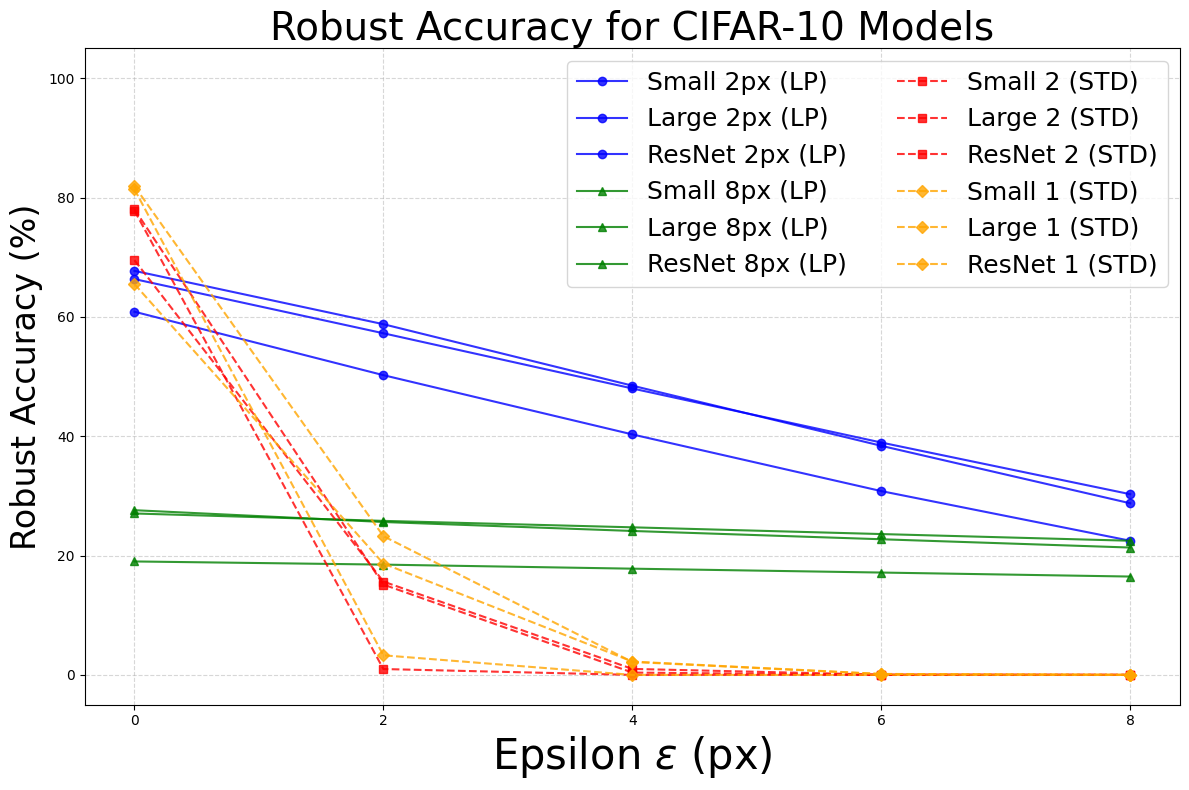
\includegraphics[width=0.85\linewidth]{images/Single model performance.png}
    \caption{Robust accuracy (\%) of LP- and standard-trained CIFAR-10 models under varying perturbation budgets $\epsilon$. LP-trained models (2px and 8px) are shown in blue/green solid lines with circle/triangle markers; standard-trained models (different checkpoints) are shown in red/orange dashed lines with square/diamond markers.}
\label{fig:robust_accuracy}

\end{figure}

\paragraph{Influence of LP Training on Robust Accuracy}  
Figure~\ref{fig:robust_accuracy} illustrates the robust accuracy trends of twelve individual models evaluated on the CIFAR-10 test set under progressively increasing adversarial perturbation budgets $\epsilon$, ranging from clean accuracy ($0px$) to a maximum perturbation setting.

Key observations include:  
\begin{itemize}
    \item \textbf{Trade-off between clean accuracy and robustness:} LP-trained models exhibit lower clean accuracy (accuracy at $\epsilon=0$) compared to standard-trained models. This reflects the known trade-off where improving certified robustness through LP training often entails some loss in clean accuracy~\cite{wong2018provable}.
    \item \textbf{Effect of training perturbation budget within LP models:} Among LP models, those trained with a smaller perturbation budget ($2\text{px}$) generally achieve higher accuracy under low perturbations but degrade more rapidly as $\epsilon$ increases, showing a near-linear decline. Conversely, LP models trained with a larger budget ($8\text{px}$) maintain more stable accuracy across perturbation levels, exhibiting less sensitivity to stronger attacks despite starting with lower clean accuracy.
    \item \textbf{Comparative robustness:} Standard-trained models demonstrate significantly poorer robustness, with sharp drops in accuracy even at the smallest evaluated perturbation budget ($2\text{px}$), and nearly zero accuracy at larger budgets. This stark contrast emphasizes the effectiveness of LP training in defending against adversarial perturbations.
\end{itemize}

These trends highlight two fundamental trade-offs in adversarial robustness research:  
(1) \textit{Robustness vs. clean accuracy trade-off}, where certified robust training methods sacrifice some clean accuracy for robustness gains;  
(2) \textit{Perturbation budget trade-off}, where training with larger budgets increases robustness but at the cost of clean accuracy and overall accuracy under small perturbations.



\begin{figure}[htbp]
    \centering
    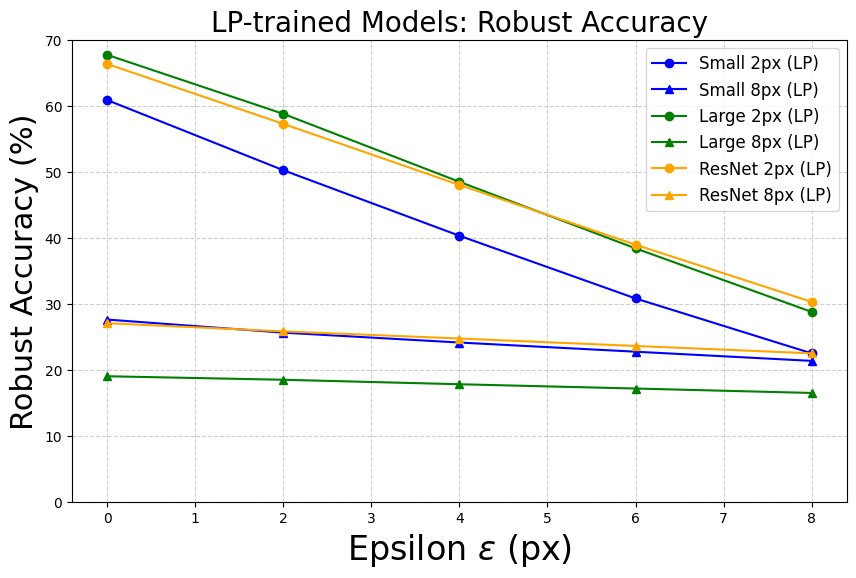
\includegraphics[width=0.80\linewidth]{images/LP_MODEL_STRUCTURE.png}
    \caption{Robust accuracy (\%) of LP-trained models on CIFAR-10 under varying perturbation budgets $\epsilon$ for different architectures: Small, Large, and ResNet. Each line corresponds to a model trained with either 2px or 8px perturbation budget.}
    \label{fig:lp_model_structure}
\end{figure}

\begin{figure}[htbp]
    \centering
    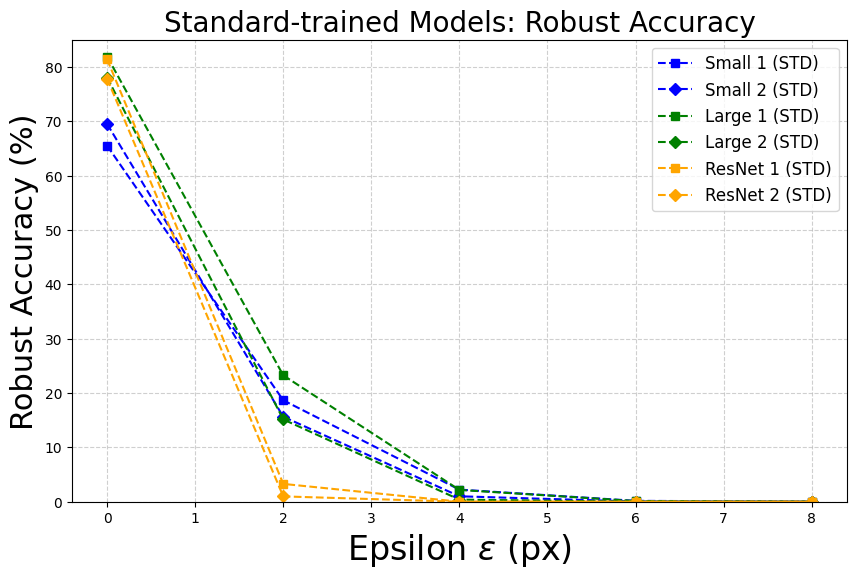
\includegraphics[width=0.80\linewidth]{images/STD_MODEL_STRUCTURE.png}
    \caption{Robust accuracy (\%) of standard-trained models on CIFAR-10 under varying perturbation budgets $\epsilon$ for different architectures: Small, Large, and ResNet.}
    \label{fig:std_model_structure}
\end{figure}

\paragraph{Model Structure Impact on Robust Accuracy}

Figures~\ref{fig:lp_model_structure} and~\ref{fig:std_model_structure} illustrate the robust accuracy of different model architectures (Small, Large, ResNet) under varying perturbation budgets $\epsilon$ for LP-trained and standard-trained models respectively.

For the \textbf{LP-trained models} (Figure~\ref{fig:lp_model_structure}), we observe the following trends:

\begin{itemize}
    \item Under the \textbf{2px training budget}, the \textit{Small} model consistently achieves approximately 8\% lower robust accuracy compared to the \textit{Large} and \textit{ResNet} architectures. This suggests that for smaller perturbation budgets, the \textit{Small} model’s capacity might limit its robustness.
    \item When trained under the \textbf{8px perturbation budget}, the \textit{Large} model exhibits roughly 8\% lower robust accuracy than both the \textit{Small} and \textit{ResNet} models. This may indicate that the \textit{Large} model struggles to maintain accuracy when trained on larger perturbations, potentially due to over-regularization or optimization difficulties at higher budgets.
    \item Across both training budgets, the \textit{ResNet} model shows relatively stable and competitive robustness, closely matching or slightly outperforming the \textit{Small} model under the 8px budget.
\end{itemize}

These observations highlight a nuanced trade-off where model size and architecture influence robustness differently depending on the adversarial training perturbation scale.

For the \textbf{standard-trained models} (Figure~\ref{fig:std_model_structure}), the trends differ significantly:

\begin{itemize}
    \item The \textit{ResNet} models suffer the steepest decline in robust accuracy as perturbation size increases, indicating lower inherent robustness under adversarial attacks without specialized training.
    \item The \textit{Large} model follows with the second fastest decline, while the \textit{Small} model maintains the slowest rate of degradation, albeit at generally low robust accuracy levels.
\end{itemize}

In summary, the impact of model structure on robustness is highly context-dependent. LP training significantly boosts robustness overall, but the choice of architecture and training perturbation budget jointly determine the precise robustness profile. Conversely, without robust training, smaller models show relatively better stability against increasing perturbations despite lower absolute accuracy.






\subsection{Ensemble Methods vs. Best Single Model}
\indent

To evaluate the performance and characteristics of different ensemble methods under adversarial perturbations, we adopt the threat model described in Section~\ref{sec:threat model} and consider multiple perturbation budgets. 
Following the recommendations in~\cite{zhang2024evaluating}, and to mitigate the risk of obfuscated gradients that can lead to misleading robustness evaluations, all attacks are performed on the surrogate model introduced in Section~\ref{sec:surrogate model}.
The experimental results are presented in Tables~\ref{tab:ensemble_lp_compact} and~\ref{tab:ensemble_std_compact}.


In addition to standard robust accuracy metrics, the \texttt{CrossMax-Ambiguous} method includes two extra indicators: 
\emph{Unique predictions only}, the robust accuracy when the prediction set contains exactly one label; 
and \emph{Prediction set contains label}, the robust accuracy when the ground-truth label is included in the prediction set. 
The detailed methodology for \texttt{CrossMax} and its variants has been described in Section~\ref{sec:crossmax}.

\begin{table}[H]
\centering
\small
\caption{Comparison of Robust Accuracy(\%) between ensemble methods and the best single LP-trained model on CIFAR-10 (LP models). 
    ``Best Single'' is the best robust accuracy among all individual models. 
    The ensemble methods are compared against the best single LP-trained model. 
    Detailed per-model results are available in Table~\ref{tab:lp_robust_accuracy_detailed}.}
\label{tab:ensemble_lp_compact}
\begin{tabular}{lccccc}
\toprule
\textbf{Model / Method} & \textbf{Clean (0 px)} & \textbf{2 px} & \textbf{4 px} & \textbf{6 px} & \textbf{8 px} \\
\midrule
Best Single (LP)            & 67.71 & 58.77 & 48.47 & 38.94 & 30.28 \\
\midrule
CrossMax-Exact (LP)         & 55.17 & 53.29 & 48.61 & 43.20 & 37.21 \\
CrossMax-Ambiguous (LP)     & \underline{\textbf{70.40}} & \underline{\textbf{68.49}} & \underline{\textbf{63.91}} & \underline{\textbf{57.73}} & \underline{\textbf{51.68}} \\
\quad Unique predictions only & 68.20 & 65.60 & 60.50 & 53.74 & 46.38 \\
\quad Prediction set contains label & 72.09 & 70.74 & 66.59 & 60.85 & 55.76 \\
\midrule
Average Voting (LP)         & 64.96 & 56.94 & 48.71 & 40.02 & 32.29 \\
Majority Voting (LP)        & 59.84 & 57.56 & 52.40 & 45.15 & 38.65 \\
\bottomrule
\end{tabular}
\end{table}


\begin{table}[H]
\centering
\small
\caption{Comparison of Robust Accuracy(\%) between ensemble methods and the best single model on CIFAR-10 (STD models).  
    ``Best Single'' is the best accuracy among all individual models. 
    The ensemble methods are compared against the best single STD model. 
    Detailed per-model results are available in Table~\ref{tab:std_robust_accuracy_detailed}.}
\label{tab:ensemble_std_compact}
\begin{tabular}{lccccc}
\toprule
\textbf{Model / Method} & \textbf{Clean (0 px)} & \textbf{2 px} & \textbf{4 px} & \textbf{6 px} & \textbf{8 px} \\
\midrule
Best Single (STD)            & 81.90 & 23.25 &  2.23 &  0.16 &  0.02 \\
\midrule
CrossMax-Exact (STD)         & 80.81 & 43.56 & 16.58 &  6.58 &  3.41 \\
CrossMax-Ambiguous (STD)     & \underline{\textbf{88.47}} & \underline{\textbf{64.42}} & \underline{\textbf{39.92}} & \underline{\textbf{23.46}} & \underline{\textbf{14.34}} \\
\quad Unique predictions only & 89.86 & 49.91 &  4.88 &  0.16 &  0.08 \\
\quad Prediction set contains label & 84.25 & 82.04 & 81.98 & 76.73 & 69.32 \\
\midrule
Average Voting (STD)         & 83.22 & 26.86 &  2.37 &  0.01 &  0.01 \\
Majority Voting (STD)        & 82.03 & 42.59 & 14.74 &  4.91 &  2.55 \\
\bottomrule
\end{tabular}
\end{table}

\begin{figure}[htbp]
    \centering
    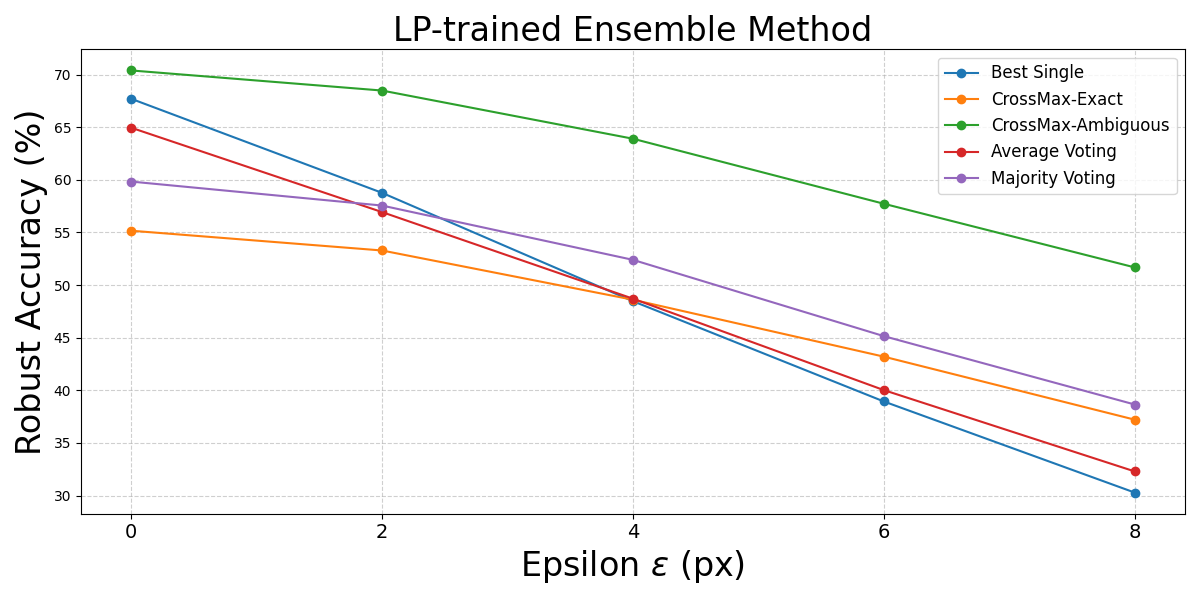
\includegraphics[width=1.0\textwidth]{images/Ensemble LP Performance.png}
    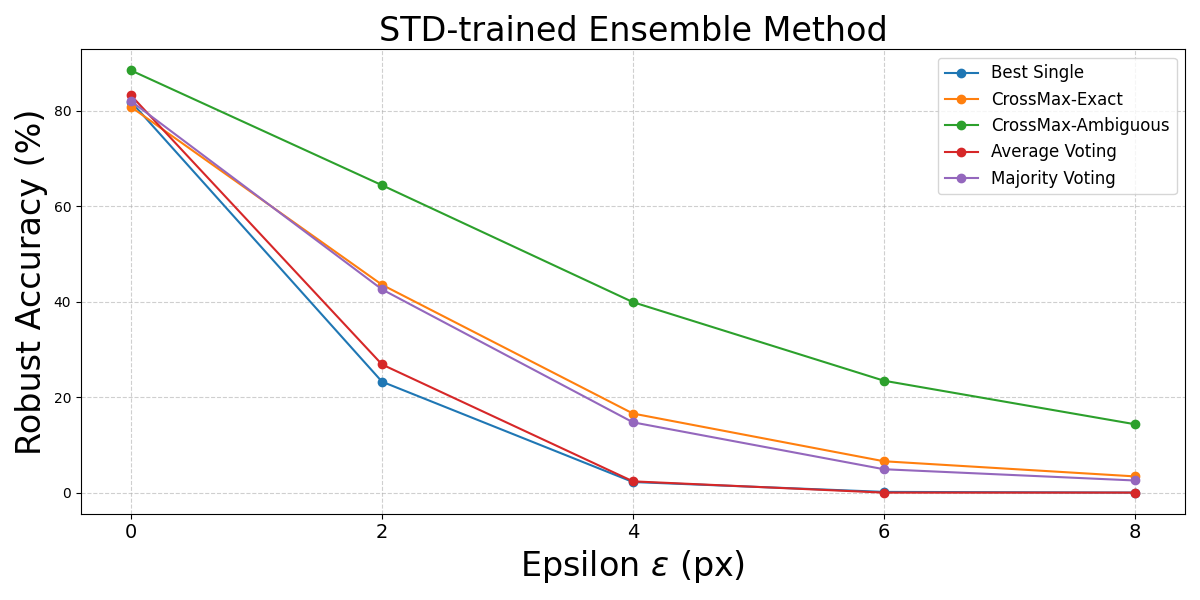
\includegraphics[width=1.0\textwidth]{images/Ensemble STD Performance.png}
    \caption{
    Comparison of ensemble methods vs. the best single model under varying perturbation budgets. 
    Top: ensembles of LP-trained models; Bottom: ensembles of Standard-trained models.
    }

    \label{fig:ensemble_performance}
\end{figure}

\paragraph{Robust Accuracy in Ensemble Methods}
From Tables~\ref{tab:ensemble_lp_compact},  \ref{tab:ensemble_std_compact} and Figure~\ref{fig:ensemble_performance}, we can observe distinct behaviors of the ensemble methods under different perturbation budgets for LP and STD models. For LP models, CrossMax-Ambiguous consistently achieves the highest robust accuracy across all $\epsilon$ values, outperforming the best single model by a notable margin (e.g., +2.69\% at $\epsilon=0$, +21.4\% at $\epsilon=8\mathrm{px}$). The improvement is especially evident at larger perturbation budgets, where the robust accuracy drop is mitigated. The ``Prediction set contains label'' metric remains consistently higher than both the best single model and other ensemble baselines, suggesting that CrossMax-Ambiguous provides more informative prediction sets even when not fully certain. On the other hand, Average Voting and Majority Voting show mixed results: Majority Voting tends to outperform Average Voting at larger $\epsilon$.  
It is worth noting that CrossMax-Exact does not perform as well as expected, particularly under small perturbations where model agreement is relatively high. Compared to CrossMax-Ambiguous, its robust accuracy suffers from the limitation of selecting a single prediction from sets that may contain multiple plausible labels. This shortcoming will be further discussed in Chapter~\ref{chap:conclusion & future work}. Although CrossMax-Ambiguous achieves the best performance in all scenarios, this is obtained under a relaxed prediction requirement. To better understand the characteristics and behavior of its prediction sets, we conducted additional experiments and analyses in the subsequent sections.

For STD models, the advantage of ensemble methods is even more pronounced under adversarial perturbations. CrossMax-Exact offers substantial gains over the best single model starting from $\epsilon=2\mathrm{px}$ (e.g., +20.31\% at $\epsilon=2\mathrm{px}$, +3.39\% at $\epsilon=8\mathrm{px}$). CrossMax-Ambiguous shows the strongest robustness, with large improvements over the best single model across all perturbation budgets, especially in high $\epsilon$ regimes (e.g., +14.32\% absolute robust accuracy at $\epsilon=8\mathrm{px}$). The ``Prediction set contains label'' robust accuracy remains extremely high ($>69\%$) even when the base robust accuracy drops close to zero, indicating its capacity to maintain label coverage under severe perturbations. In contrast, traditional voting methods (Average and Majority) perform significantly worse, particularly for large perturbations, where their robust accuracy approaches that of random guessing.

Overall, CrossMax-Ambiguous emerges as the most effective ensemble method for both LP and STD settings, providing both higher robust accuracy and better label coverage. These results highlight the potential of set-based ensemble predictions in improving robustness under large perturbations, where conventional single-model or simple voting ensembles fail.


\subsection{CrossMax-Ambiguous Prediction Set Size}
\indent

Table~\ref{tab:crossmax_ambiguous} summarizes the average size of the ambiguous prediction sets produced by the CrossMax aggregation method under different perturbation levels for both LP-trained and standard (STD) models. Here, the ambiguous prediction set size refers to the number of classes remaining in the top-$k$ candidates after the CrossMax filtering process, which reflects the model's uncertainty structure from a multi-model perspective.

\begin{table}[h]
\centering
\caption{Average CrossMax-Ambiguous prediction set size under different perturbation budgets.}
\label{tab:crossmax_ambiguous}
\begin{tabular}{c|cc}
\hline
\textbf{Epsilon} & \textbf{LP Model} & \textbf{STD Model} \\
\hline
Clean (0px)   & 1.5768 & 1.2577 \\
2px   & 1.5743 & 1.4665 \\
4px   & 1.5740 & 1.4630 \\
6px   & 1.5737 & 1.3105 \\
8px   & 1.5798 & 1.2117 \\
\hline
\end{tabular}
\end{table}

From Table~\ref{tab:crossmax_ambiguous}, we observe that:
\begin{itemize}
    \item For LP models, the ambiguous set size remains remarkably stable ($\approx 1.57$) across all perturbation levels, indicating that the CrossMax aggregation preserves a consistent level of decision ambiguity even under strong adversarial perturbations.
    \item For STD models, the ambiguous set size is lower than that of LP models when $\epsilon=0$, suggesting higher confidence in clean settings. However, it increases significantly for moderate perturbations ($\epsilon=2,4$) before dropping again at higher perturbations ($\epsilon=6,8$). This pattern suggests that STD models become more uncertain under small-to-moderate attacks, but their predictions collapse to fewer candidate classes under stronger perturbations, potentially due to overconfident misclassification.
\end{itemize}





\subsection{Diversity and Confidence Analysis}  
\label{sec:diversity-confidence-analysis}
\indent

In this section, we analyze and compare the diversity and confidence characteristics of ensembles constructed from two types of base models: LP-trained and standard-trained. We examine how these metrics evolve under varying strengths of adversarial perturbations, providing insights into the robustness mechanisms at play.

Specifically, we first quantify the prediction diversity and ensemble confidence of individual models inside the ensemble as the perturbation budget increases, highlighting differences in their behavior and resilience (Section~\ref{sec:diversity-confidence}). Next, we investigate the CrossMax ensemble method’s ability to produce a unique (single) prediction under different perturbation levels, analyzing how the perturbation strength impacts the CrossMax Confidence score. This offers a nuanced view of prediction ambiguity and certainty in adversarial scenarios.

To contextualize and deepen our understanding, we further compare CrossMax-derived confidence with several traditional ensemble uncertainty and confidence metrics, including softmax-based confidence, prediction entropy, mutual information, and vote agreement. Through this comparative analysis, we aim to reveal correlations and distinctions among these measures and their implications for ensemble robustness.

\begin{table}[htbp]
\centering
\small
\caption{Ensemble Diversity and Confidence Metrics for \textbf{LP-trained} models under varying perturbation budgets.}
\label{tab:diversity_confidence_lp}
\begin{tabular}{lccccc}
\toprule
\textbf{Perturbation} & \textbf{CrossMax Conf.} & \textbf{Diversity} & \textbf{Softmax Conf.} & \textbf{Entropy} & \textbf{Mutual Info.} \\
\midrule
Clean(0px)   & 0.4343 & 0.0057 & 0.3831 & 1.9068 & 0.2259 \\
2px   & 0.4375 & 0.0057 & 0.3823 & 1.9076 & 0.2252 \\
4px   & 0.4400 & 0.0057 & 0.3796 & 1.9107 & 0.2229 \\
6px   & 0.4393 & 0.0057 & 0.3747 & 1.9170 & 0.2188 \\
8px   & 0.4349 & 0.0058 & 0.3689 & 1.9253 & 0.2139 \\
\bottomrule
\end{tabular}
\end{table}


\vspace{1em}

\begin{table}[htbp]
\centering
\small
\caption{Ensemble Diversity and Confidence Metrics for \textbf{STD} models under varying perturbation budgets.}
\label{tab:diversity_confidence_std}
\begin{tabular}{lccccc}
\toprule
\textbf{Perturbation} & \textbf{CrossMax Conf.} & \textbf{Diversity} & \textbf{Softmax Conf.} & \textbf{Entropy} & \textbf{Mutual Info.} \\
\midrule
Clean(0px)   & 0.7517 & 0.0026 & 0.7704 & 0.8133 & 0.1733 \\
2px   & 0.5484 & 0.0038 & 0.7551 & 0.9116 & 0.2459 \\
4px   & 0.5455 & 0.0038 & 0.7771 & 0.8978 & 0.2947 \\
6px   & 0.6957 & 0.0028 & 0.8161 & 0.7547 & 0.2506 \\
8px   & 0.7940 & 0.0021 & 0.8448 & 0.6328 & 0.2019 \\
\bottomrule
\end{tabular}
\end{table}






\paragraph{Diversity and Confidence in LP vs. Standard Ensembles}

Tables~\ref{tab:diversity_confidence_std} and~\ref{tab:diversity_confidence_lp} summarize key ensemble metrics for standard-trained (STD) and LP-trained models under varying perturbation budgets. 

We observe that the LP-trained ensembles consistently exhibit higher prediction diversity than the STD-trained ones across all perturbation levels, with diversity values around 0.0057–0.0058 compared to the STD’s lower range of 0.0021–0.0038. This indicates that LP training encourages more heterogeneous network predictions inside ensemble model, which can contribute to robustness against adversarial transferability.

In contrast, confidence metrics such as CrossMax Confidence and Softmax Confidence are notably higher for the STD ensembles, especially at larger perturbations (e.g., at 8px, CrossMax Confidence reaches 0.7940 for STD vs. 0.4349 for LP). Correspondingly, the STD models tend to have lower prediction entropy, suggesting more confident and sharper ensemble predictions compared to LP models, which maintain high entropy values (~about 1.9), indicative of greater uncertainty.

MI, reflecting epistemic uncertainty and model disagreement, exhibits smaller variation in LP-trained ensembles compared to standard ensembles, suggesting more consistent behavior among networks inside ensemble models despite their robustness-oriented training. Similarly, entropy values for LP-trained ensembles remain consistently high (around 1.90–1.92) across perturbation budgets, indicating uniformly distributed predictions and limited confidence shifts. In contrast, entropy in standard ensembles fluctuates sharply (from 0.81 at clean inputs to 0.91 and then dropping to 0.63), highlighting greater volatility in predictive confidence under adversarial perturbations.

However, as observed from Tables~\ref{tab:ensemble_lp_compact} and \ref{tab:ensemble_std_compact}, high confidence does not necessarily imply reliable predictions. This “confidence” can be substantially misleading when all models are extensively fooled by strong attacks. For instance, under the 8px attack on the STD ensemble, despite the model exhibiting high self-confidence in its predictions (CrossMax Confidence of 0.7940), the actual ensemble performance deteriorates drastically, with majority voting accuracy plummeting to only 2.55\%. This highlights the gap between confidence measures and true robustness under adversarial conditions.


\paragraph{CrossMax Confidence and Softmax Confidence under Perturbations}

To further explore ensemble confidence dynamics, we compare CrossMax Confidence with Softmax Confidence as perturbation strength varies, using the two figures shown in Figures~\ref{fig:softmax_confidence} and ~\ref{fig:crossmax_confidence}. Both plots illustrate the trend of confidence scores for LP-trained and standard-trained ensembles under increasing adversarial budgets.

We observe that the more robust LP-trained ensembles maintain remarkably stable confidence scores across both metrics, with fluctuations on the order of $10^{-2}$. In contrast, the STD-trained ensembles, which are more susceptible to adversarial perturbations, show notably larger variability in confidence. For both CrossMax and Softmax Confidence, the STD models exhibit a non-monotonic trend: confidence first decreases as attacks grow stronger, then increases again when perturbations become large enough to deceive most networks inside the ensemble model simultaneously.

Interestingly, this characteristic pattern is more pronounced in CrossMax Confidence than in Softmax Confidence. According to Table~\ref{tab:diversity_confidence_std}, the absolute change in Softmax Confidence across perturbations is approximately 0.0897, whereas CrossMax Confidence demonstrates a larger absolute difference of 0.2485. This suggests that CrossMax Confidence captures the ensemble’s shifting certainty more sensitively under adversarial conditions, potentially providing a more informative measure of robustness compared to traditional softmax-based confidence.



\begin{figure}[H]
    \centering
    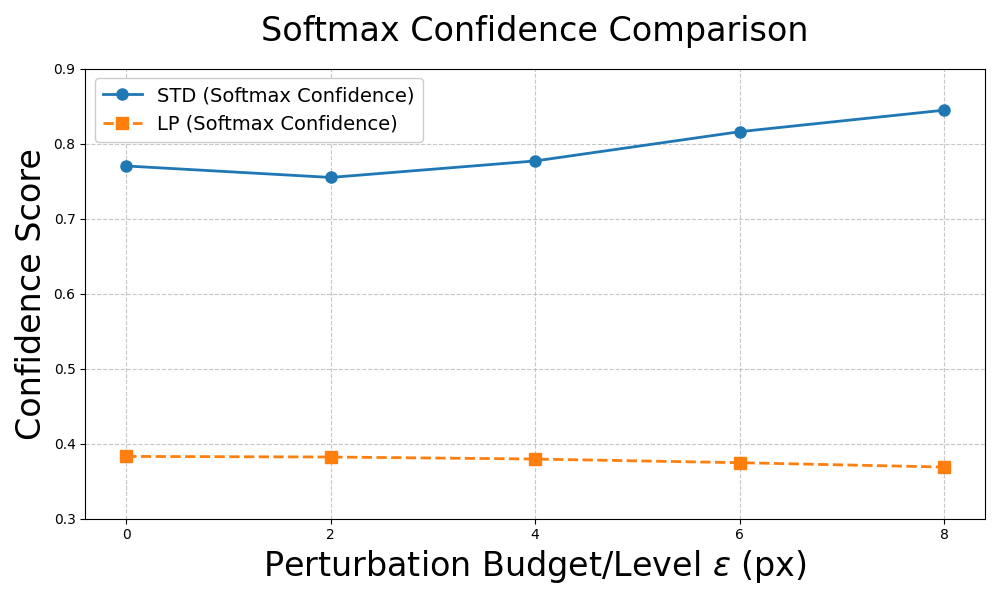
\includegraphics[width=0.8\linewidth]{images/SoftMax Confidence.png}
    \caption{Softmax Confidence scores for LP-trained and STD-trained ensembles as perturbation budget increases.}
    \label{fig:softmax_confidence}
\end{figure}

\begin{figure}[H]
    \centering
    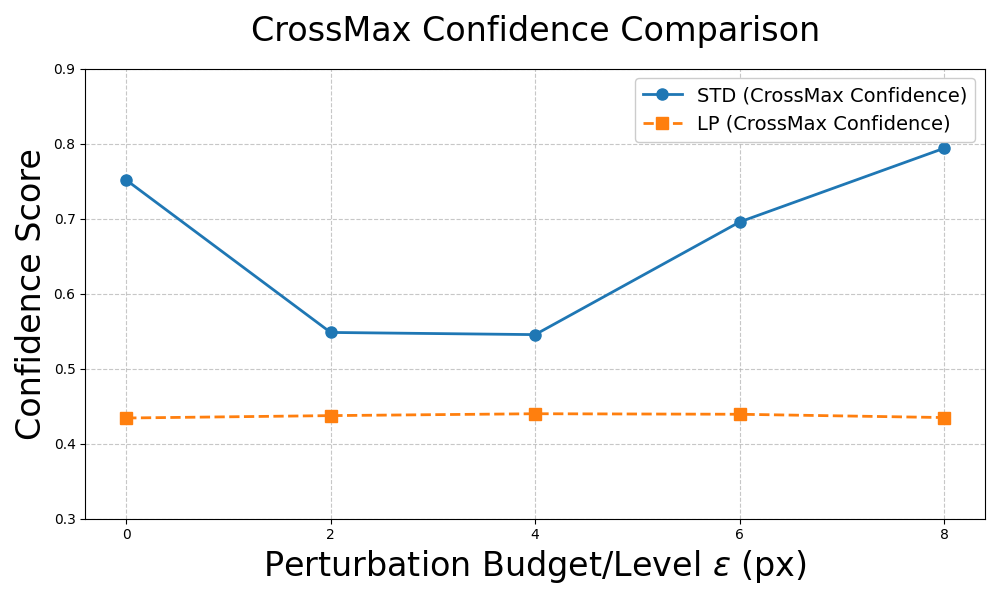
\includegraphics[width=0.8\linewidth]{images/CrossMax Confidence.png}
    \caption{CrossMax Confidence scores for LP-trained and STD-trained ensembles as perturbation budget increases.}
    \label{fig:crossmax_confidence}
\end{figure}


\section{Discussion}
\label{sec:discussion}
\indent

This section synthesizes the experimental findings and interprets their implications for ensemble robustness under adversarial perturbations, with a particular focus on differences between LP-trained and standard-trained models, the impact of model architectures, and the effectiveness of various ensemble strategies and confidence metrics.

\paragraph{Robustness and Accuracy Trade-offs in LP Training}

Consistent with prior literature~\cite{li2023sok}, LP-trained models exhibit a well-known trade-off between clean accuracy and certified robustness. Our results demonstrate that LP training improves adversarial robustness substantially compared to standard training, especially at higher perturbation budgets. However, this robustness gain comes at the cost of reduced clean accuracy, highlighting a fundamental tension in adversarial defenses. Moreover, the perturbation budget used during training critically shapes the robustness profile: models trained with smaller budgets perform better under light perturbations but degrade quickly as attacks intensify, while models trained with larger budgets show more stable performance across all perturbations despite lower clean accuracy.

\paragraph{Model Architecture Effects on Robustness}

Our analysis reveals that the impact of model architecture on robustness is nuanced and depends heavily on the training regime. For LP-trained models, ResNet architectures generally achieve a better balance of robustness and stability across perturbations, while Large models underperform at higher budgets possibly due to over-regularization or optimization challenges. Conversely, in the absence of robust training, smaller models appear more stable against increasing perturbations, though their absolute robust accuracy remains low. This suggests that architectural complexity interacts with training strategy to influence robustness characteristics in non-trivial ways.

\paragraph{Ensemble Methods and Their Robustness Benefits}

Across both LP and standard training, set-based ensemble methods CrossMax-Ambiguous, outperform traditional averaging or majority voting approaches in robust accuracy, especially at higher perturbation levels. This indicates that relaxing the ensemble prediction to a set of plausible labels can effectively mitigate the sharp accuracy drop-off caused by strong adversarial attacks. Notably, CrossMax-Exact underperforms when perturbations are small and networks agreement inside the ensemble model is high, likely due to its restrictive single-label output. The advantage of CrossMax-Ambiguous highlights the potential of incorporating prediction ambiguity into ensemble robustness strategies.

\paragraph{Ambiguity in CrossMax Ensemble Predictions}

The ambiguous prediction set size produced by CrossMax aggregation reveals contrasting behaviors between LP and standard ensembles. LP-trained ensembles maintain a stable ambiguous set size (~around 1.57 classes), even as perturbations increase, suggesting preserved decision diversity and calibrated uncertainty. In contrast, standard-trained ensembles exhibit a non-monotonic trend in ambiguity: initial high confidence on clean data gives way to increased ambiguity at moderate perturbations, followed by a collapse to fewer candidate classes under strong attacks. This pattern reflects a breakdown in confidence calibration and growing overconfidence in erroneous predictions as attacks intensify.

\paragraph{Diversity and Confidence Metrics under Perturbations}

LP-trained ensembles consistently exhibit higher prediction diversity than standard-trained ones, reflecting more heterogeneous network outputs inside the ensemble model which may aid robustness against transferable adversarial perturbations. Standard-trained ensembles show higher CrossMax and Softmax confidence, especially at large perturbations, but this confidence is often misleading. For example, under strong attacks, the standard ensemble's CrossMax Confidence remains high while actual accuracy plummets, evidencing overconfident yet unreliable predictions.

Further analysis of confidence dynamics shows that LP-trained ensembles maintain remarkably stable confidence across perturbation strengths, with minimal fluctuations in both CrossMax and Softmax metrics. In contrast, standard-trained ensembles experience pronounced confidence oscillations: confidence dips as perturbations grow stronger, then rises again when most networks inside the ensemble model are fooled. This non-monotonic behavior is more evident in CrossMax Confidence than Softmax Confidence, suggesting that CrossMax metrics may better capture the ensemble’s shifting uncertainty and provide a more sensitive indicator of robustness under adversarial conditions.

\paragraph{Summary}

Overall, our study underscores the complex interplay between training strategies, model architecture, ensemble methods, and confidence measures in shaping adversarial robustness. LP training and sophisticated ensemble approaches like CrossMax-Ambiguous improve robustness but highlight the need for careful confidence calibration and ambiguity-aware predictions. The observed limitations of standard confidence metrics and traditional ensemble voting suggest promising directions for future research, including the development of more reliable confidence indicators and adaptive ensemble aggregation techniques tailored for adversarial resilience.
% ----------------- CHAPTER 5 -----------------
\chapter{Conclusions and Future Work}
\label{chap:conclusion & future work}

\paragraph{Conclusion}
This work systematically evaluated ensemble robustness under adversarial perturbations, comparing LP-trained and standard-trained models, different architectures, and ensemble aggregation methods such as CrossMax. A key practical insight is that users of ensemble models can monitor the volatility of \textit{CrossMax Confidence} as a diagnostic for adversarial sensitivity: ensembles exhibiting large fluctuations in CrossMax Confidence across perturbation levels tend to have weaker robustness, while more robust ensembles show remarkably stable CrossMax Confidence scores throughout.

Our experiments further reveal that while CrossMax-Ambiguous effectively leverages prediction ambiguity to improve robustness, the related method CrossMax-Exact underperforms due to the difficulty of selecting the optimal final prediction from ambiguous prediction sets. The current heuristic for choosing a prediction approximates random selection, limiting performance gains.

\paragraph{Future Work}
For future work, inspired by the cascading approach proposed by Wong et al.~\cite{wong2018scaling}, we propose to train specialized, robust binary classifiers dedicated to disambiguating prediction sets generated by CrossMax-Ambiguous. Because these binary models only need to be robust for two-class decisions rather than full multi-class classification, their training cost is lower and certified robustness easier to achieve. Leveraging these robust binary discriminators in a cascade to resolve ambiguous prediction sets promises to enhance the accuracy and robustness of CrossMax-Exact ensembles significantly. This direction opens a promising avenue for combining certified robustness techniques with ensemble uncertainty modeling to further advance provable defenses in adversarial settings.
% ----------------- APPENDIX ------------------

\chapter*{Appendices} \addcontentsline{toc}{chapter}{Appendices} 
\renewcommand{\thesection}{\Alph{section}} 

\section{Pseudocode of the original CrossMax Ensemble}
\label{alg:crossmax}
\begin{algorithm}
\caption{CrossMax Ensemble (Pseudocode)~\cite{fort2024ensemble}}
\begin{algorithmic}
\Require $Z_1, Z_2, \dots, Z_M \in \mathbb{R}^{B \times C}$ (logits from $M$ models)
\State Stack logits into $Z \in \mathbb{R}^{B \times M \times C}$
\State Normalize $Z$ by subtracting max logit across classes per predictor
\State Normalize $Z$ by subtracting max logit across predictors per class
\State Compute $k$-th largest logit per class across models
\Ensure Class with highest $k$-th (e.g., $k=2$) largest logit
\end{algorithmic}
\end{algorithm}


\section{Bound on the Size of CrossMax Prediction Sets}
\label{appendix:crossmax-bound}

Consider the CrossMax aggregation with $M$ predictors and $C$ classes.  
Let the logits matrix be
\[
\mathbf{Z} \in \mathbb{R}^{M \times C},
\]
where the $i$-th row $\mathbf{z}_i$ corresponds to the logits from predictor $i$, and $z_{i,c}$ denotes the logit for class $c$.

\paragraph{Step 1: Removing predictor dominance.}  
For each predictor $i$, subtract its maximum logit over all classes:
\[
\tilde{\mathbf{z}}_{i,c} = \mathbf{z}_{i,c} - \max_{c'} \mathbf{z}_{i,c'}.
\]
After this normalization, each predictor’s logits contain exactly one zero (corresponding to the original maximum), while the remaining entries are strictly negative (ignoring ties). Thus, there are exactly $M$ zeros in the normalized logits matrix, one per predictor.

\paragraph{Step 2: Removing class dominance.}  
For each class $c$, subtract the maximum logit among all predictors:
\[
\hat{\mathbf{z}}_{i,c} = \tilde{\mathbf{z}}_{i,c} - \max_{j} \tilde{\mathbf{z}}_{j,c}.
\]
Since all entries $\tilde{z}_{i,c} \leq 0$, the maximum within a class is always non-positive. Two cases arise:
\begin{itemize}
    \item If all $\tilde{\mathbf{z}}_{i,c} < 0$, then the maximum is strictly negative. After subtraction, one predictor attains zero for class $c$, and the rest are negative.
    \item If there exists some predictor $i$ with $\tilde{\mathbf{z}}_{i,c}=0$, then $\max_j \tilde{\mathbf{z}}_{j,c}=0$, so the logits for that class remain unchanged.
\end{itemize}

\paragraph{Step 3: $k$-th max aggregation.}  
CrossMax selects the $k$-th largest value across predictors for each class:
\[
s_c = \operatorname{k\text{-}max}_{i} \ \hat{\mathbf{z}}_{i,c}.
\]
A class $c$ belongs to the prediction set if
\[
s_c = 0.
\]
This requires at least $k$ predictors to have $\hat{\mathbf{z}}_{i,c} = 0$ for that class.

\paragraph{Bound on prediction set size.}  
Since there are exactly $M$ zeros in total (one per predictor after Step 1), the maximal number of classes that can satisfy $s_c=0$ is bounded by
\[
\left\lfloor \frac{M}{k} \right\rfloor.
\]

\paragraph{Interpretation.}  
This shows that the size of the CrossMax prediction set is \textbf{bounded above by} $\lfloor M/k \rfloor$.  
In our experiments with $M=6$ predictors and $k=2$, the prediction set size can never exceed $3$.  
Hence, the CrossMax rule inherently prevents excessively large ambiguous outputs, limiting uncertainty by design.
\hfill $\square$



% ----------------- REFERENCES -----------------
\bibliographystyle{IEEEtran}
\bibliography{references}

\end{document}
